\documentclass[twoside]{book}

% Packages required by doxygen
\usepackage{fixltx2e}
\usepackage{calc}
\usepackage{doxygen}
\usepackage[export]{adjustbox} % also loads graphicx
\usepackage{graphicx}
\usepackage[utf8]{inputenc}
\usepackage{makeidx}
\usepackage{multicol}
\usepackage{multirow}
\PassOptionsToPackage{warn}{textcomp}
\usepackage{textcomp}
\usepackage[nointegrals]{wasysym}
\usepackage[table]{xcolor}

% Font selection
\usepackage[T1]{fontenc}
\usepackage[scaled=.90]{helvet}
\usepackage{courier}
\usepackage{amssymb}
\usepackage{sectsty}
\renewcommand{\familydefault}{\sfdefault}
\allsectionsfont{%
  \fontseries{bc}\selectfont%
  \color{darkgray}%
}
\renewcommand{\DoxyLabelFont}{%
  \fontseries{bc}\selectfont%
  \color{darkgray}%
}
\newcommand{\+}{\discretionary{\mbox{\scriptsize$\hookleftarrow$}}{}{}}

% Page & text layout
\usepackage{geometry}
\geometry{%
  a4paper,%
  top=2.5cm,%
  bottom=2.5cm,%
  left=2.5cm,%
  right=2.5cm%
}
\tolerance=750
\hfuzz=15pt
\hbadness=750
\setlength{\emergencystretch}{15pt}
\setlength{\parindent}{0cm}
\setlength{\parskip}{3ex plus 2ex minus 2ex}
\makeatletter
\renewcommand{\paragraph}{%
  \@startsection{paragraph}{4}{0ex}{-1.0ex}{1.0ex}{%
    \normalfont\normalsize\bfseries\SS@parafont%
  }%
}
\renewcommand{\subparagraph}{%
  \@startsection{subparagraph}{5}{0ex}{-1.0ex}{1.0ex}{%
    \normalfont\normalsize\bfseries\SS@subparafont%
  }%
}
\makeatother

% Headers & footers
\usepackage{fancyhdr}
\pagestyle{fancyplain}
\fancyhead[LE]{\fancyplain{}{\bfseries\thepage}}
\fancyhead[CE]{\fancyplain{}{}}
\fancyhead[RE]{\fancyplain{}{\bfseries\leftmark}}
\fancyhead[LO]{\fancyplain{}{\bfseries\rightmark}}
\fancyhead[CO]{\fancyplain{}{}}
\fancyhead[RO]{\fancyplain{}{\bfseries\thepage}}
\fancyfoot[LE]{\fancyplain{}{}}
\fancyfoot[CE]{\fancyplain{}{}}
\fancyfoot[RE]{\fancyplain{}{\bfseries\scriptsize Generated by Doxygen }}
\fancyfoot[LO]{\fancyplain{}{\bfseries\scriptsize Generated by Doxygen }}
\fancyfoot[CO]{\fancyplain{}{}}
\fancyfoot[RO]{\fancyplain{}{}}
\renewcommand{\footrulewidth}{0.4pt}
\renewcommand{\chaptermark}[1]{%
  \markboth{#1}{}%
}
\renewcommand{\sectionmark}[1]{%
  \markright{\thesection\ #1}%
}

% Indices & bibliography
\usepackage{natbib}
\usepackage[titles]{tocloft}
\setcounter{tocdepth}{3}
\setcounter{secnumdepth}{5}
\makeindex

% Hyperlinks (required, but should be loaded last)
\usepackage{ifpdf}
\ifpdf
  \usepackage[pdftex,pagebackref=true]{hyperref}
\else
  \usepackage[ps2pdf,pagebackref=true]{hyperref}
\fi
\hypersetup{%
  colorlinks=true,%
  linkcolor=blue,%
  citecolor=blue,%
  unicode%
}

% Custom commands
\newcommand{\clearemptydoublepage}{%
  \newpage{\pagestyle{empty}\cleardoublepage}%
}

\usepackage{caption}
\captionsetup{labelsep=space,justification=centering,font={bf},singlelinecheck=off,skip=4pt,position=top}

%===== C O N T E N T S =====

\begin{document}

% Titlepage & ToC
\hypersetup{pageanchor=false,
             bookmarksnumbered=true,
             pdfencoding=unicode
            }
\pagenumbering{alph}
\begin{titlepage}
\vspace*{7cm}
\begin{center}%
{\Large A Graph Model of Intermodal Transportation Networks }\\
\vspace*{1cm}
{\large Generated by Doxygen 1.8.12}\\
\end{center}
\end{titlepage}
\clearemptydoublepage
\pagenumbering{roman}
\tableofcontents
\clearemptydoublepage
\pagenumbering{arabic}
\hypersetup{pageanchor=true}

%--- Begin generated contents ---
\chapter{Class Index}
\section{Class List}
Here are the classes, structs, unions and interfaces with brief descriptions\+:\begin{DoxyCompactList}
\item\contentsline{section}{\hyperlink{class_connection}{Connection} }{\pageref{class_connection}}{}
\item\contentsline{section}{\hyperlink{class_edge}{Edge} }{\pageref{class_edge}}{}
\item\contentsline{section}{\hyperlink{class_edge_type}{Edge\+Type} }{\pageref{class_edge_type}}{}
\item\contentsline{section}{\hyperlink{class_geographic_coords}{Geographic\+Coords} }{\pageref{class_geographic_coords}}{}
\item\contentsline{section}{\hyperlink{class_graph}{Graph} }{\pageref{class_graph}}{}
\item\contentsline{section}{\hyperlink{class_graph_viewer}{Graph\+Viewer} }{\pageref{class_graph_viewer}}{}
\item\contentsline{section}{\hyperlink{class_node}{Node} }{\pageref{class_node}}{}
\item\contentsline{section}{\hyperlink{structnode__greater__than}{node\+\_\+greater\+\_\+than} }{\pageref{structnode__greater__than}}{}
\item\contentsline{section}{\hyperlink{structnode__pair__greater__than}{node\+\_\+pair\+\_\+greater\+\_\+than} }{\pageref{structnode__pair__greater__than}}{}
\item\contentsline{section}{\hyperlink{class_point}{Point} }{\pageref{class_point}}{}
\item\contentsline{section}{\hyperlink{class_road}{Road} }{\pageref{class_road}}{}
\item\contentsline{section}{\hyperlink{class_transport}{Transport} }{\pageref{class_transport}}{}
\end{DoxyCompactList}

\chapter{Class Documentation}
\hypertarget{class_connection}{}\section{Connection Class Reference}
\label{class_connection}\index{Connection@{Connection}}


{\ttfamily \#include $<$connection.\+h$>$}



Collaboration diagram for Connection\+:\nopagebreak
\begin{figure}[H]
\begin{center}
\leavevmode
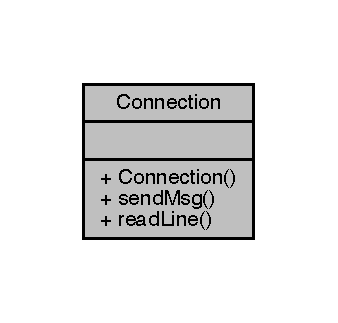
\includegraphics[width=162pt]{class_connection__coll__graph}
\end{center}
\end{figure}
\subsection*{Public Member Functions}
\begin{DoxyCompactItemize}
\item 
\hyperlink{class_connection_a8089476d48ba545f44e691cd4bd0278d}{Connection} (short port)
\item 
bool \hyperlink{class_connection_a4b9f6db1fb42fc9857f829fa0bc52e6e}{send\+Msg} (string msg)
\item 
string \hyperlink{class_connection_a1df16b436751b686d96c24ca0c498659}{read\+Line} ()
\end{DoxyCompactItemize}


\subsection{Constructor \& Destructor Documentation}
\hypertarget{class_connection_a8089476d48ba545f44e691cd4bd0278d}{}\label{class_connection_a8089476d48ba545f44e691cd4bd0278d} 
\index{Connection@{Connection}!Connection@{Connection}}
\index{Connection@{Connection}!Connection@{Connection}}
\subsubsection{\texorpdfstring{Connection()}{Connection()}}
{\footnotesize\ttfamily Connection\+::\+Connection (\begin{DoxyParamCaption}\item[{short}]{port }\end{DoxyParamCaption})}



\subsection{Member Function Documentation}
\hypertarget{class_connection_a1df16b436751b686d96c24ca0c498659}{}\label{class_connection_a1df16b436751b686d96c24ca0c498659} 
\index{Connection@{Connection}!read\+Line@{read\+Line}}
\index{read\+Line@{read\+Line}!Connection@{Connection}}
\subsubsection{\texorpdfstring{read\+Line()}{readLine()}}
{\footnotesize\ttfamily string Connection\+::read\+Line (\begin{DoxyParamCaption}{ }\end{DoxyParamCaption})}

\hypertarget{class_connection_a4b9f6db1fb42fc9857f829fa0bc52e6e}{}\label{class_connection_a4b9f6db1fb42fc9857f829fa0bc52e6e} 
\index{Connection@{Connection}!send\+Msg@{send\+Msg}}
\index{send\+Msg@{send\+Msg}!Connection@{Connection}}
\subsubsection{\texorpdfstring{send\+Msg()}{sendMsg()}}
{\footnotesize\ttfamily bool Connection\+::send\+Msg (\begin{DoxyParamCaption}\item[{string}]{msg }\end{DoxyParamCaption})}



The documentation for this class was generated from the following files\+:\begin{DoxyCompactItemize}
\item 
\hyperlink{connection_8h}{connection.\+h}\item 
\hyperlink{connection_8cpp}{connection.\+cpp}\end{DoxyCompactItemize}

\hypertarget{class_edge}{}\section{Edge Class Reference}
\label{class_edge}\index{Edge@{Edge}}


{\ttfamily \#include $<$Edge.\+hpp$>$}

\subsection*{Public Member Functions}
\begin{DoxyCompactItemize}
\item 
\hyperlink{class_edge_ae9995324a7970fb53ff489a518cac211}{Edge} (\hyperlink{class_node}{Node} $\ast$origin, \hyperlink{class_node}{Node} $\ast$dest, \hyperlink{class_road}{Road} $\ast$road, \hyperlink{class_transport_a1879cecfed0d4238e5a7af6d085db317}{Transport\+::\+Type} type=Transport\+::\+F\+O\+OT)
\item 
unsigned \hyperlink{class_edge_ac047f6b04f3cb9b590058a2a96e303e7}{get\+Cost} () const
\item 
edge\+\_\+id \hyperlink{class_edge_afb88989f2a1b21bdd1d5aaa4054486c3}{get\+ID} () const
\item 
\hyperlink{class_node}{Node} $\ast$ \hyperlink{class_edge_af2cd0f7cba34228f76c4b20a84a2de9d}{get\+Dest} () const
\item 
\hyperlink{class_node}{Node} $\ast$ \hyperlink{class_edge_a04719c702ae24dcfbce3874a573ca360}{get\+Origin} () const
\item 
\hyperlink{class_road}{Road} $\ast$ \hyperlink{class_edge_ae967ccaa1db4dba903ccfb3c55be9bc5}{get\+Road} () const
\item 
float \hyperlink{class_edge_ae96241bc7956c47dba61f7a0cfec01c3}{get\+Length} () const
\item 
float \hyperlink{class_edge_a873322923fa6340e17edb39b923f7d61}{get\+Weight} () const
\item 
\hyperlink{class_transport_a1879cecfed0d4238e5a7af6d085db317}{Transport\+::\+Type} \hyperlink{class_edge_ad36b220701f80c199f9b2ed7bb79a22f}{get\+Type} () const
\end{DoxyCompactItemize}
\subsection*{Friends}
\begin{DoxyCompactItemize}
\item 
ostream \& \hyperlink{class_edge_a4ba287cbdc78be9ec49dd1b67291039b}{operator$<$$<$} (ostream \&out, const \hyperlink{class_edge}{Edge} \&e)
\end{DoxyCompactItemize}


\subsection{Detailed Description}
A class used to represent a \hyperlink{class_edge}{Edge} in a \hyperlink{class_graph}{Graph}, therefore used to join two Nodes. Every \hyperlink{class_edge}{Edge} has a unique ID, used to represent itself; a \hyperlink{class_node}{Node} as Origin and a \hyperlink{class_node}{Node} as Destiny. Every \hyperlink{class_edge}{Edge} is also associated to a \hyperlink{class_road}{Road}, that contains more information about it. 

\subsection{Constructor \& Destructor Documentation}
\hypertarget{class_edge_ae9995324a7970fb53ff489a518cac211}{}\label{class_edge_ae9995324a7970fb53ff489a518cac211} 
\index{Edge@{Edge}!Edge@{Edge}}
\index{Edge@{Edge}!Edge@{Edge}}
\subsubsection{\texorpdfstring{Edge()}{Edge()}}
{\footnotesize\ttfamily Edge\+::\+Edge (\begin{DoxyParamCaption}\item[{\hyperlink{class_node}{Node} $\ast$}]{origin,  }\item[{\hyperlink{class_node}{Node} $\ast$}]{dest,  }\item[{\hyperlink{class_road}{Road} $\ast$}]{road,  }\item[{\hyperlink{class_transport_a1879cecfed0d4238e5a7af6d085db317}{Transport\+::\+Type}}]{type = {\ttfamily Transport\+:\+:FOOT} }\end{DoxyParamCaption})}

\hyperlink{class_edge}{Edge}\textquotesingle{}s constructor. Creates a \hyperlink{class_edge}{Edge} with a given origin \hyperlink{class_node}{Node}, destiny \hyperlink{class_node}{Node} and associated Rode. A transport mean may be provided, otherwise defaults to F\+O\+OT (walking).


\begin{DoxyParams}{Parameters}
{\em origin} & \hyperlink{class_edge}{Edge}\textquotesingle{}s origin \hyperlink{class_node}{Node}. \\
\hline
{\em dest} & \hyperlink{class_edge}{Edge}\textquotesingle{}s destiny \hyperlink{class_node}{Node}. \\
\hline
{\em road} & Rode associated to the \hyperlink{class_edge}{Edge} that is being created. \\
\hline
{\em type} & Type of transport used to traverse the \hyperlink{class_edge}{Edge} that is being created. \\
\hline
\end{DoxyParams}


\subsection{Member Function Documentation}
\hypertarget{class_edge_ac047f6b04f3cb9b590058a2a96e303e7}{}\label{class_edge_ac047f6b04f3cb9b590058a2a96e303e7} 
\index{Edge@{Edge}!get\+Cost@{get\+Cost}}
\index{get\+Cost@{get\+Cost}!Edge@{Edge}}
\subsubsection{\texorpdfstring{get\+Cost()}{getCost()}}
{\footnotesize\ttfamily unsigned Edge\+::get\+Cost (\begin{DoxyParamCaption}{ }\end{DoxyParamCaption}) const}

Getter for \hyperlink{class_edge}{Edge}\textquotesingle{}s cost. Corresponds to the monetary cost it takes to traverse this \hyperlink{class_edge}{Edge}.

\begin{DoxyReturn}{Returns}
The cost of traversing this \hyperlink{class_edge}{Edge}. 
\end{DoxyReturn}
\hypertarget{class_edge_af2cd0f7cba34228f76c4b20a84a2de9d}{}\label{class_edge_af2cd0f7cba34228f76c4b20a84a2de9d} 
\index{Edge@{Edge}!get\+Dest@{get\+Dest}}
\index{get\+Dest@{get\+Dest}!Edge@{Edge}}
\subsubsection{\texorpdfstring{get\+Dest()}{getDest()}}
{\footnotesize\ttfamily \hyperlink{class_node}{Node} $\ast$ Edge\+::get\+Dest (\begin{DoxyParamCaption}{ }\end{DoxyParamCaption}) const}

Getter for \hyperlink{class_edge}{Edge}\textquotesingle{}s destiny \hyperlink{class_node}{Node}.

\begin{DoxyReturn}{Returns}
\hyperlink{class_edge}{Edge}\textquotesingle{}s destiny \hyperlink{class_node}{Node}. 
\end{DoxyReturn}
\hypertarget{class_edge_afb88989f2a1b21bdd1d5aaa4054486c3}{}\label{class_edge_afb88989f2a1b21bdd1d5aaa4054486c3} 
\index{Edge@{Edge}!get\+ID@{get\+ID}}
\index{get\+ID@{get\+ID}!Edge@{Edge}}
\subsubsection{\texorpdfstring{get\+I\+D()}{getID()}}
{\footnotesize\ttfamily edge\+\_\+id Edge\+::get\+ID (\begin{DoxyParamCaption}{ }\end{DoxyParamCaption}) const}

Getter for \hyperlink{class_edge}{Edge}\textquotesingle{}s ID. The ID is used to represent an \hyperlink{class_edge}{Edge}, since there are no two Edges with the same ID.

\begin{DoxyReturn}{Returns}
The \hyperlink{class_edge}{Edge}\textquotesingle{}s ID. 
\end{DoxyReturn}
\hypertarget{class_edge_ae96241bc7956c47dba61f7a0cfec01c3}{}\label{class_edge_ae96241bc7956c47dba61f7a0cfec01c3} 
\index{Edge@{Edge}!get\+Length@{get\+Length}}
\index{get\+Length@{get\+Length}!Edge@{Edge}}
\subsubsection{\texorpdfstring{get\+Length()}{getLength()}}
{\footnotesize\ttfamily float Edge\+::get\+Length (\begin{DoxyParamCaption}{ }\end{DoxyParamCaption}) const}

Getter for \hyperlink{class_edge}{Edge}\textquotesingle{}s length. Corresponds to the physical distance between the two Nodes linked by this edge.

\begin{DoxyReturn}{Returns}
Distance of the two nodes linked by this \hyperlink{class_edge}{Edge}. 
\end{DoxyReturn}
\hypertarget{class_edge_a04719c702ae24dcfbce3874a573ca360}{}\label{class_edge_a04719c702ae24dcfbce3874a573ca360} 
\index{Edge@{Edge}!get\+Origin@{get\+Origin}}
\index{get\+Origin@{get\+Origin}!Edge@{Edge}}
\subsubsection{\texorpdfstring{get\+Origin()}{getOrigin()}}
{\footnotesize\ttfamily \hyperlink{class_node}{Node} $\ast$ Edge\+::get\+Origin (\begin{DoxyParamCaption}{ }\end{DoxyParamCaption}) const}

Getter for \hyperlink{class_edge}{Edge}\textquotesingle{}s origin \hyperlink{class_node}{Node}.

\begin{DoxyReturn}{Returns}
\hyperlink{class_edge}{Edge}\textquotesingle{}s origin \hyperlink{class_node}{Node}. 
\end{DoxyReturn}
\hypertarget{class_edge_ae967ccaa1db4dba903ccfb3c55be9bc5}{}\label{class_edge_ae967ccaa1db4dba903ccfb3c55be9bc5} 
\index{Edge@{Edge}!get\+Road@{get\+Road}}
\index{get\+Road@{get\+Road}!Edge@{Edge}}
\subsubsection{\texorpdfstring{get\+Road()}{getRoad()}}
{\footnotesize\ttfamily \hyperlink{class_road}{Road} $\ast$ Edge\+::get\+Road (\begin{DoxyParamCaption}{ }\end{DoxyParamCaption}) const}

Getter for \hyperlink{class_edge}{Edge}\textquotesingle{}s \hyperlink{class_road}{Road}. \hyperlink{class_road}{Road}\textquotesingle{}s contain additional information regarding the Edges.

\begin{DoxyReturn}{Returns}
\hyperlink{class_road}{Road} associated to this \hyperlink{class_edge}{Edge}. 
\end{DoxyReturn}
\hypertarget{class_edge_ad36b220701f80c199f9b2ed7bb79a22f}{}\label{class_edge_ad36b220701f80c199f9b2ed7bb79a22f} 
\index{Edge@{Edge}!get\+Type@{get\+Type}}
\index{get\+Type@{get\+Type}!Edge@{Edge}}
\subsubsection{\texorpdfstring{get\+Type()}{getType()}}
{\footnotesize\ttfamily \hyperlink{class_transport_a1879cecfed0d4238e5a7af6d085db317}{Transport\+::\+Type} Edge\+::get\+Type (\begin{DoxyParamCaption}{ }\end{DoxyParamCaption}) const}

Getter for \hyperlink{class_edge}{Edge}\textquotesingle{}s type of transport. The type of transport used can be one out of three options\+: bus, subway or walking.

\begin{DoxyReturn}{Returns}
The type of transport used to traverse this \hyperlink{class_edge}{Edge}. 
\end{DoxyReturn}
\hypertarget{class_edge_a873322923fa6340e17edb39b923f7d61}{}\label{class_edge_a873322923fa6340e17edb39b923f7d61} 
\index{Edge@{Edge}!get\+Weight@{get\+Weight}}
\index{get\+Weight@{get\+Weight}!Edge@{Edge}}
\subsubsection{\texorpdfstring{get\+Weight()}{getWeight()}}
{\footnotesize\ttfamily float Edge\+::get\+Weight (\begin{DoxyParamCaption}{ }\end{DoxyParamCaption}) const}

Getter for \hyperlink{class_edge}{Edge}\textquotesingle{}s weight. Corresponds to the average time (in seconds -\/ SI unit) needed to traverse this \hyperlink{class_edge}{Edge}.

\begin{DoxyReturn}{Returns}
Average time needed to traverse this \hyperlink{class_edge}{Edge}. 
\end{DoxyReturn}


\subsection{Friends And Related Function Documentation}
\hypertarget{class_edge_a4ba287cbdc78be9ec49dd1b67291039b}{}\label{class_edge_a4ba287cbdc78be9ec49dd1b67291039b} 
\index{Edge@{Edge}!operator$<$$<$@{operator$<$$<$}}
\index{operator$<$$<$@{operator$<$$<$}!Edge@{Edge}}
\subsubsection{\texorpdfstring{operator$<$$<$}{operator<<}}
{\footnotesize\ttfamily ostream\& operator$<$$<$ (\begin{DoxyParamCaption}\item[{ostream \&}]{out,  }\item[{const \hyperlink{class_edge}{Edge} \&}]{e }\end{DoxyParamCaption})\hspace{0.3cm}{\ttfamily [friend]}}

Overload of operator $<$$<$ for Class \hyperlink{class_edge}{Edge}. Writes the \hyperlink{class_edge}{Edge} passed as second argument to the outstream passed as first argument.


\begin{DoxyParams}{Parameters}
{\em out} & Output stream to write to. \\
\hline
{\em e} & \hyperlink{class_edge}{Edge} the will be written.\\
\hline
\end{DoxyParams}
\begin{DoxyReturn}{Returns}
The output stream, therefore allowing chaining. 
\end{DoxyReturn}


The documentation for this class was generated from the following files\+:\begin{DoxyCompactItemize}
\item 
Edge.\+hpp\item 
Edge.\+cpp\end{DoxyCompactItemize}

\hypertarget{class_edge_type}{}\section{Edge\+Type Class Reference}
\label{class_edge_type}\index{Edge\+Type@{Edge\+Type}}


{\ttfamily \#include $<$edgetype.\+h$>$}

\subsection*{Static Public Attributes}
\begin{DoxyCompactItemize}
\item 
\hypertarget{class_edge_type_a6533cc56d05c288a550b9980b66c9317}{}\label{class_edge_type_a6533cc56d05c288a550b9980b66c9317} 
static const int {\bfseries U\+N\+D\+I\+R\+E\+C\+T\+ED} = 0
\item 
\hypertarget{class_edge_type_a903017a534f2818c2d17145e4ae0321c}{}\label{class_edge_type_a903017a534f2818c2d17145e4ae0321c} 
static const int {\bfseries D\+I\+R\+E\+C\+T\+ED} = 1
\end{DoxyCompactItemize}


\subsection{Detailed Description}
Classe que enumera os tipos de arestas. Usar Edge\+Type.\+U\+N\+D\+I\+R\+E\+C\+T\+ED para uma aresta sem direcção, ou Edge\+Type.\+D\+I\+R\+E\+C\+T\+ED para uma aresta dirigida. 

The documentation for this class was generated from the following file\+:\begin{DoxyCompactItemize}
\item 
edgetype.\+h\end{DoxyCompactItemize}

\hypertarget{class_geographic_coords}{}\section{Geographic\+Coords Class Reference}
\label{class_geographic_coords}\index{Geographic\+Coords@{Geographic\+Coords}}


{\ttfamily \#include $<$Coordinates.\+hpp$>$}



Collaboration diagram for Geographic\+Coords\+:
\nopagebreak
\begin{figure}[H]
\begin{center}
\leavevmode
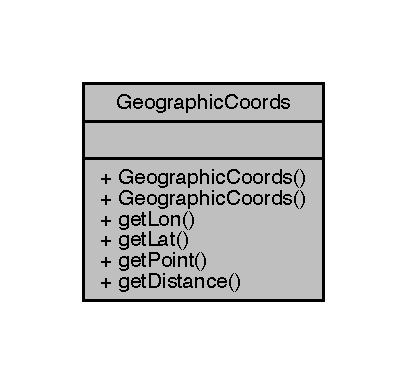
\includegraphics[width=195pt]{class_geographic_coords__coll__graph}
\end{center}
\end{figure}
\subsection*{Public Member Functions}
\begin{DoxyCompactItemize}
\item 
\hyperlink{class_geographic_coords_a6e58da78d507551dc7a6c39e6ffb33b3}{Geographic\+Coords} ()=default
\item 
\hyperlink{class_geographic_coords_a5db8168e8754a1eb2d13e3d2c8318cb4}{Geographic\+Coords} (float lat, float lon)
\item 
float \hyperlink{class_geographic_coords_a4e59f2e3ea261e73c33014368770ad21}{get\+Lon} () const
\item 
float \hyperlink{class_geographic_coords_ab2fa1d7cde50be2a00c297caa302297a}{get\+Lat} () const
\item 
\hyperlink{class_point}{Point} \hyperlink{class_geographic_coords_aa333be28efcee6d8da24adabe5cd5594}{get\+Point} (pair$<$ float, float $>$ lat\+Range, pair$<$ float, float $>$ lon\+Range) const
\end{DoxyCompactItemize}
\subsection*{Static Public Member Functions}
\begin{DoxyCompactItemize}
\item 
static float \hyperlink{class_geographic_coords_a25f3ba7791c305b8620bb0ef8adac156}{get\+Distance} (const \hyperlink{class_geographic_coords}{Geographic\+Coords} \&p1, const \hyperlink{class_geographic_coords}{Geographic\+Coords} \&p2)
\end{DoxyCompactItemize}


\subsection{Detailed Description}
Class used to represent Geographical Coordinates. Therefore, every Coordinate is represented with longitude and latitude. 

\subsection{Constructor \& Destructor Documentation}
\hypertarget{class_geographic_coords_a6e58da78d507551dc7a6c39e6ffb33b3}{}\label{class_geographic_coords_a6e58da78d507551dc7a6c39e6ffb33b3} 
\index{Geographic\+Coords@{Geographic\+Coords}!Geographic\+Coords@{Geographic\+Coords}}
\index{Geographic\+Coords@{Geographic\+Coords}!Geographic\+Coords@{Geographic\+Coords}}
\subsubsection{\texorpdfstring{Geographic\+Coords()}{GeographicCoords()}\hspace{0.1cm}{\footnotesize\ttfamily [1/2]}}
{\footnotesize\ttfamily Geographic\+Coords\+::\+Geographic\+Coords (\begin{DoxyParamCaption}{ }\end{DoxyParamCaption})\hspace{0.3cm}{\ttfamily [default]}}

Explicit Default constructor \hypertarget{class_geographic_coords_a5db8168e8754a1eb2d13e3d2c8318cb4}{}\label{class_geographic_coords_a5db8168e8754a1eb2d13e3d2c8318cb4} 
\index{Geographic\+Coords@{Geographic\+Coords}!Geographic\+Coords@{Geographic\+Coords}}
\index{Geographic\+Coords@{Geographic\+Coords}!Geographic\+Coords@{Geographic\+Coords}}
\subsubsection{\texorpdfstring{Geographic\+Coords()}{GeographicCoords()}\hspace{0.1cm}{\footnotesize\ttfamily [2/2]}}
{\footnotesize\ttfamily Geographic\+Coords\+::\+Geographic\+Coords (\begin{DoxyParamCaption}\item[{float}]{lat,  }\item[{float}]{lon }\end{DoxyParamCaption})}

Geographic Coordinates constructor. Creates a Geographic Coordinate with the given Latitude and Longitude.


\begin{DoxyParams}{Parameters}
{\em lat} & Latitude value, in radians. \\
\hline
{\em lon} & Longitude value, in radians. \\
\hline
\end{DoxyParams}


\subsection{Member Function Documentation}
\hypertarget{class_geographic_coords_a25f3ba7791c305b8620bb0ef8adac156}{}\label{class_geographic_coords_a25f3ba7791c305b8620bb0ef8adac156} 
\index{Geographic\+Coords@{Geographic\+Coords}!get\+Distance@{get\+Distance}}
\index{get\+Distance@{get\+Distance}!Geographic\+Coords@{Geographic\+Coords}}
\subsubsection{\texorpdfstring{get\+Distance()}{getDistance()}}
{\footnotesize\ttfamily float Geographic\+Coords\+::get\+Distance (\begin{DoxyParamCaption}\item[{const \hyperlink{class_geographic_coords}{Geographic\+Coords} \&}]{p1,  }\item[{const \hyperlink{class_geographic_coords}{Geographic\+Coords} \&}]{p2 }\end{DoxyParamCaption})\hspace{0.3cm}{\ttfamily [static]}}

Mathematical formula for the projected (2D) distance between two points in space, defined by their Geographic Coordinates. \href{https://en.wikipedia.org/wiki/Geographical_distance#Spherical_Earth_projected_to_a_plane}{\tt https\+://en.\+wikipedia.\+org/wiki/\+Geographical\+\_\+distance\#\+Spherical\+\_\+\+Earth\+\_\+projected\+\_\+to\+\_\+a\+\_\+plane}


\begin{DoxyParams}{Parameters}
{\em p1} & Geographic Coordinate to be used in the calculus. \\
\hline
{\em p2} & Geographic Coordinate to be used in the calculus.\\
\hline
\end{DoxyParams}
\begin{DoxyReturn}{Returns}
the distance between the two Geographic Coordinates.
\end{DoxyReturn}
Mathematical formula for the projected (2D) distance between two points in space, defined by their Geographic Coordinates. \href{https://en.wikipedia.org/wiki/Geographical_distance#Spherical_Earth_projected_to_a_plane}{\tt https\+://en.\+wikipedia.\+org/wiki/\+Geographical\+\_\+distance\#\+Spherical\+\_\+\+Earth\+\_\+projected\+\_\+to\+\_\+a\+\_\+plane} \hypertarget{class_geographic_coords_ab2fa1d7cde50be2a00c297caa302297a}{}\label{class_geographic_coords_ab2fa1d7cde50be2a00c297caa302297a} 
\index{Geographic\+Coords@{Geographic\+Coords}!get\+Lat@{get\+Lat}}
\index{get\+Lat@{get\+Lat}!Geographic\+Coords@{Geographic\+Coords}}
\subsubsection{\texorpdfstring{get\+Lat()}{getLat()}}
{\footnotesize\ttfamily float Geographic\+Coords\+::get\+Lat (\begin{DoxyParamCaption}{ }\end{DoxyParamCaption}) const}

Getter for latitude value of the Geographic Coordinate.

\begin{DoxyReturn}{Returns}
latitude value. 
\end{DoxyReturn}
\hypertarget{class_geographic_coords_a4e59f2e3ea261e73c33014368770ad21}{}\label{class_geographic_coords_a4e59f2e3ea261e73c33014368770ad21} 
\index{Geographic\+Coords@{Geographic\+Coords}!get\+Lon@{get\+Lon}}
\index{get\+Lon@{get\+Lon}!Geographic\+Coords@{Geographic\+Coords}}
\subsubsection{\texorpdfstring{get\+Lon()}{getLon()}}
{\footnotesize\ttfamily float Geographic\+Coords\+::get\+Lon (\begin{DoxyParamCaption}{ }\end{DoxyParamCaption}) const}

Getter for longitude value of the Geographic Coordinate.

\begin{DoxyReturn}{Returns}
longitude value. 
\end{DoxyReturn}
\hypertarget{class_geographic_coords_aa333be28efcee6d8da24adabe5cd5594}{}\label{class_geographic_coords_aa333be28efcee6d8da24adabe5cd5594} 
\index{Geographic\+Coords@{Geographic\+Coords}!get\+Point@{get\+Point}}
\index{get\+Point@{get\+Point}!Geographic\+Coords@{Geographic\+Coords}}
\subsubsection{\texorpdfstring{get\+Point()}{getPoint()}}
{\footnotesize\ttfamily \hyperlink{class_point}{Point} Geographic\+Coords\+::get\+Point (\begin{DoxyParamCaption}\item[{pair$<$ float, float $>$}]{lat\+Range,  }\item[{pair$<$ float, float $>$}]{lon\+Range }\end{DoxyParamCaption}) const}

Parser from a Geographic Coordinate to a \hyperlink{class_point}{Point}. This parser takes in consideration the Latitude and Longitude range, so that it can map the 2D Referential.


\begin{DoxyParams}{Parameters}
{\em lat\+Range} & Pair of floats containing the Latitude range, where the first element is the minimum and the second the maximum. \\
\hline
{\em lon\+Range} & Pair of floats containing the Longitude range, where the first element is the minimum and the second the maximum.\\
\hline
\end{DoxyParams}
\begin{DoxyReturn}{Returns}
the \hyperlink{class_point}{Point} gotten from parsing the Geographic Coordinate. 
\end{DoxyReturn}


The documentation for this class was generated from the following files\+:\begin{DoxyCompactItemize}
\item 
\hyperlink{_coordinates_8hpp}{Coordinates.\+hpp}\item 
\hyperlink{_coordinates_8cpp}{Coordinates.\+cpp}\end{DoxyCompactItemize}

\hypertarget{class_graph}{}\section{Graph Class Reference}
\label{class_graph}\index{Graph@{Graph}}


{\ttfamily \#include $<$Graph.\+hpp$>$}

\subsection*{Public Member Functions}
\begin{DoxyCompactItemize}
\item 
\hyperlink{class_graph_aadb341e62a5548bf406c05834aa187da}{Graph} (istream \&nodes, istream \&edges, istream \&roads, istream \&subway, istream \&bus)
\item 
\hyperlink{class_graph_a7a3f0c7dceffa85819bf122c49fd973c}{Graph} (const \hyperlink{class_graph}{Graph} \&obj)
\item 
\hyperlink{class_graph_a902c5b3eacb66d60752525ab23297a95}{$\sim$\+Graph} ()
\item 
node\+\_\+id \hyperlink{class_graph_aec10981cceac64d033e2e0de5b34c995}{get\+Node\+I\+D\+From\+Parser\+ID} (int parser\+ID) const
\item 
unordered\+\_\+map$<$ node\+\_\+id, \hyperlink{class_node}{Node} $\ast$ $>$ \hyperlink{class_graph_aa64f6696d40b6a8e0d92df399ed11310}{get\+Nodes} () const
\item 
unordered\+\_\+map$<$ edge\+\_\+id, \hyperlink{class_edge}{Edge} $\ast$ $>$ \hyperlink{class_graph_a7dd776ad17a9d14b14f044373c79a9bc}{get\+Edges} () const
\item 
unordered\+\_\+map$<$ road\+\_\+id, \hyperlink{class_road}{Road} $\ast$ $>$ \hyperlink{class_graph_a101befc9baedb7dc3aaa714c968dc943}{get\+Roads} () const
\item 
void \hyperlink{class_graph_a819fb225997f026a192ec5df1b17df84}{dijkstra\+Shortest\+Path} (node\+\_\+id src\+\_\+id, node\+\_\+id dest\+\_\+id=0)
\item 
void \hyperlink{class_graph_a0fc41701fa170ab69282ae8a571fdc04}{dijkstra\+Shortest\+Path} (\hyperlink{class_node}{Node} $\ast$src, \hyperlink{class_node}{Node} $\ast$destination=nullptr)
\item 
void \hyperlink{class_graph_a751cdeb2ca841f9d44d921cf1a43ddd0}{dijkstra\+Shortest\+Path} (node\+\_\+id src\+\_\+id, node\+\_\+id dest\+\_\+id, \hyperlink{class_transport_a1879cecfed0d4238e5a7af6d085db317}{Transport\+::\+Type} type, unsigned int scale=5)
\item 
void \hyperlink{class_graph_afe77f6a03cad266807c741d1a3178541}{dijkstra\+Shortest\+Path} (\hyperlink{class_node}{Node} $\ast$src, \hyperlink{class_node}{Node} $\ast$dest, \hyperlink{class_transport_a1879cecfed0d4238e5a7af6d085db317}{Transport\+::\+Type} type, unsigned int scale=5)
\item 
void \hyperlink{class_graph_a284736e6b467032dce3bfd69213c31f0}{dijkstra\+Shortest\+Path\+With\+Max\+Cost} (node\+\_\+id src\+\_\+id, node\+\_\+id dest\+\_\+id, unsigned max\+Cost)
\item 
vector$<$ \hyperlink{class_node}{Node} $\ast$ $>$ \hyperlink{class_graph_ae4c66eaf1b29f53bf90ad6266baa6819}{get\+Path} (node\+\_\+id src\+\_\+id, node\+\_\+id dest\+\_\+id) const
\item 
vector$<$ \hyperlink{class_edge}{Edge} $\ast$ $>$ \hyperlink{class_graph_a94db80dbb52cac57e2b5d14c53e649e7}{get\+Path\+Edges} (node\+\_\+id src\+\_\+id, node\+\_\+id dest\+\_\+id) const
\item 
float \hyperlink{class_graph_adb19e47c0238b012a6a3a28bdaf855f8}{get\+Path\+Length} (node\+\_\+id src\+\_\+id, node\+\_\+id dest\+\_\+id) const
\item 
float \hyperlink{class_graph_a2d69a99fb35fee10aadc243c468ad9b2}{get\+Path\+Duration} (node\+\_\+id src\+\_\+id, node\+\_\+id dest\+\_\+id) const
\item 
unsigned \hyperlink{class_graph_a9d5ab1a266d948f146e78866ef19673d}{get\+Path\+Cost} (node\+\_\+id src\+\_\+id, node\+\_\+id dest\+\_\+id) const
\item 
void \hyperlink{class_graph_ab596c4b805ecdf622c4f3d952f894a50}{dfs} (\hyperlink{class_node}{Node} $\ast$v, vector$<$ \hyperlink{class_node}{Node} $\ast$$>$ \&res)
\end{DoxyCompactItemize}


\subsection{Detailed Description}
Class used to represent a \hyperlink{class_graph}{Graph}. Every \hyperlink{class_graph}{Graph} has a set Nodes as well as a set of Edges, linking the Nodes. The Graphs are also associated to Rodes. 

\subsection{Constructor \& Destructor Documentation}
\hypertarget{class_graph_aadb341e62a5548bf406c05834aa187da}{}\label{class_graph_aadb341e62a5548bf406c05834aa187da} 
\index{Graph@{Graph}!Graph@{Graph}}
\index{Graph@{Graph}!Graph@{Graph}}
\subsubsection{\texorpdfstring{Graph()}{Graph()}\hspace{0.1cm}{\footnotesize\ttfamily [1/2]}}
{\footnotesize\ttfamily Graph\+::\+Graph (\begin{DoxyParamCaption}\item[{istream \&}]{nodes,  }\item[{istream \&}]{edges,  }\item[{istream \&}]{roads,  }\item[{istream \&}]{subway,  }\item[{istream \&}]{bus }\end{DoxyParamCaption})}

\hyperlink{class_graph}{Graph}\textquotesingle{}s constructor. Creates a \hyperlink{class_graph}{Graph} with the data passed by the arguments input streams.


\begin{DoxyParams}{Parameters}
{\em nodes} & The input stream to read from in order to populate the Nodes\textquotesingle{} Hash map. \\
\hline
{\em edges} & The input stream to read from in order to populate the Edges\textquotesingle{} Hash map. \\
\hline
{\em roads} & The input stream to read from in order to populate the Roads\textquotesingle{} Hash map. \\
\hline
{\em subway} & The input stream containing the Edges whose mean of transport is the Subway. \\
\hline
{\em bus} & The input stream containing the Edges whose mean of transport is the Bus. \\
\hline
\end{DoxyParams}
\hyperlink{class_graph}{Graph} Pre\+Processing \hypertarget{class_graph_a7a3f0c7dceffa85819bf122c49fd973c}{}\label{class_graph_a7a3f0c7dceffa85819bf122c49fd973c} 
\index{Graph@{Graph}!Graph@{Graph}}
\index{Graph@{Graph}!Graph@{Graph}}
\subsubsection{\texorpdfstring{Graph()}{Graph()}\hspace{0.1cm}{\footnotesize\ttfamily [2/2]}}
{\footnotesize\ttfamily Graph\+::\+Graph (\begin{DoxyParamCaption}\item[{const \hyperlink{class_graph}{Graph} \&}]{obj }\end{DoxyParamCaption})}

\hyperlink{class_graph}{Graph}\textquotesingle{}s Copy constructor. Creates a new \hyperlink{class_graph}{Graph} with the same attributes as the given \hyperlink{class_graph}{Graph}.


\begin{DoxyParams}{Parameters}
{\em obj} & The \hyperlink{class_graph}{Graph} that will be copied. \\
\hline
\end{DoxyParams}
\hypertarget{class_graph_a902c5b3eacb66d60752525ab23297a95}{}\label{class_graph_a902c5b3eacb66d60752525ab23297a95} 
\index{Graph@{Graph}!````~Graph@{$\sim$\+Graph}}
\index{````~Graph@{$\sim$\+Graph}!Graph@{Graph}}
\subsubsection{\texorpdfstring{$\sim$\+Graph()}{~Graph()}}
{\footnotesize\ttfamily Graph\+::$\sim$\+Graph (\begin{DoxyParamCaption}{ }\end{DoxyParamCaption})}

\hyperlink{class_graph}{Graph}\textquotesingle{}s Destructor. Deallocates all the memory used by a \hyperlink{class_graph}{Graph}. 

\subsection{Member Function Documentation}
\hypertarget{class_graph_ab596c4b805ecdf622c4f3d952f894a50}{}\label{class_graph_ab596c4b805ecdf622c4f3d952f894a50} 
\index{Graph@{Graph}!dfs@{dfs}}
\index{dfs@{dfs}!Graph@{Graph}}
\subsubsection{\texorpdfstring{dfs()}{dfs()}}
{\footnotesize\ttfamily void Graph\+::dfs (\begin{DoxyParamCaption}\item[{\hyperlink{class_node}{Node} $\ast$}]{v,  }\item[{vector$<$ \hyperlink{class_node}{Node} $\ast$$>$ \&}]{res }\end{DoxyParamCaption})}

Runs Depth-\/\+First Search from the node pointed to by v, and pushes visited nodes into the res vector, in order.


\begin{DoxyParams}{Parameters}
{\em v} & \hyperlink{class_node}{Node} $\ast$ to start node \\
\hline
{\em res} & Vector to be filled \\
\hline
\end{DoxyParams}
\hypertarget{class_graph_a819fb225997f026a192ec5df1b17df84}{}\label{class_graph_a819fb225997f026a192ec5df1b17df84} 
\index{Graph@{Graph}!dijkstra\+Shortest\+Path@{dijkstra\+Shortest\+Path}}
\index{dijkstra\+Shortest\+Path@{dijkstra\+Shortest\+Path}!Graph@{Graph}}
\subsubsection{\texorpdfstring{dijkstra\+Shortest\+Path()}{dijkstraShortestPath()}\hspace{0.1cm}{\footnotesize\ttfamily [1/4]}}
{\footnotesize\ttfamily void Graph\+::dijkstra\+Shortest\+Path (\begin{DoxyParamCaption}\item[{node\+\_\+id}]{src\+\_\+id,  }\item[{node\+\_\+id}]{dest\+\_\+id = {\ttfamily 0} }\end{DoxyParamCaption})}

Implementation of Dijkstra\textquotesingle{}s shortest path algorithm. The shortest path will be the fastest one.


\begin{DoxyParams}{Parameters}
{\em src\+\_\+id} & The id of the origin \hyperlink{class_node}{Node}. \\
\hline
{\em dest\+\_\+id} & The id of the destiny \hyperlink{class_node}{Node}. If no value is given, it defaults to 0. \\
\hline
\end{DoxyParams}
\hypertarget{class_graph_a0fc41701fa170ab69282ae8a571fdc04}{}\label{class_graph_a0fc41701fa170ab69282ae8a571fdc04} 
\index{Graph@{Graph}!dijkstra\+Shortest\+Path@{dijkstra\+Shortest\+Path}}
\index{dijkstra\+Shortest\+Path@{dijkstra\+Shortest\+Path}!Graph@{Graph}}
\subsubsection{\texorpdfstring{dijkstra\+Shortest\+Path()}{dijkstraShortestPath()}\hspace{0.1cm}{\footnotesize\ttfamily [2/4]}}
{\footnotesize\ttfamily void Graph\+::dijkstra\+Shortest\+Path (\begin{DoxyParamCaption}\item[{\hyperlink{class_node}{Node} $\ast$}]{src,  }\item[{\hyperlink{class_node}{Node} $\ast$}]{destination = {\ttfamily nullptr} }\end{DoxyParamCaption})}

Implementation of Dijkstra\textquotesingle{}s shortest path algorithm. The shortest path will be the fastest one.


\begin{DoxyParams}{Parameters}
{\em src} & The origin \hyperlink{class_node}{Node} \\
\hline
{\em destination} & The destiny \hyperlink{class_node}{Node}. If no value is given, it defaults to nullptr. \\
\hline
\end{DoxyParams}
\hypertarget{class_graph_a751cdeb2ca841f9d44d921cf1a43ddd0}{}\label{class_graph_a751cdeb2ca841f9d44d921cf1a43ddd0} 
\index{Graph@{Graph}!dijkstra\+Shortest\+Path@{dijkstra\+Shortest\+Path}}
\index{dijkstra\+Shortest\+Path@{dijkstra\+Shortest\+Path}!Graph@{Graph}}
\subsubsection{\texorpdfstring{dijkstra\+Shortest\+Path()}{dijkstraShortestPath()}\hspace{0.1cm}{\footnotesize\ttfamily [3/4]}}
{\footnotesize\ttfamily void Graph\+::dijkstra\+Shortest\+Path (\begin{DoxyParamCaption}\item[{node\+\_\+id}]{src\+\_\+id,  }\item[{node\+\_\+id}]{dest\+\_\+id,  }\item[{\hyperlink{class_transport_a1879cecfed0d4238e5a7af6d085db317}{Transport\+::\+Type}}]{type,  }\item[{unsigned int}]{scale = {\ttfamily 5} }\end{DoxyParamCaption})}

Implementation of Dijkstra\textquotesingle{}s shortest path algorithm. The shortest path will be fastest one. This Dijkstra implementation takes into consideration the mean of \hyperlink{class_transport}{Transport} used.


\begin{DoxyParams}{Parameters}
{\em src\+\_\+id} & The id of the origin \hyperlink{class_node}{Node}. \\
\hline
{\em dest\+\_\+id} & The id of the destiny \hyperlink{class_node}{Node}. \\
\hline
{\em type} & Mean of \hyperlink{class_transport}{Transport} used. \\
\hline
{\em scale} & Mean of transport preference scale (bigger scale means higher preference). If no value is given it defaults to 5. \\
\hline
\end{DoxyParams}
\hypertarget{class_graph_afe77f6a03cad266807c741d1a3178541}{}\label{class_graph_afe77f6a03cad266807c741d1a3178541} 
\index{Graph@{Graph}!dijkstra\+Shortest\+Path@{dijkstra\+Shortest\+Path}}
\index{dijkstra\+Shortest\+Path@{dijkstra\+Shortest\+Path}!Graph@{Graph}}
\subsubsection{\texorpdfstring{dijkstra\+Shortest\+Path()}{dijkstraShortestPath()}\hspace{0.1cm}{\footnotesize\ttfamily [4/4]}}
{\footnotesize\ttfamily void Graph\+::dijkstra\+Shortest\+Path (\begin{DoxyParamCaption}\item[{\hyperlink{class_node}{Node} $\ast$}]{src,  }\item[{\hyperlink{class_node}{Node} $\ast$}]{dest,  }\item[{\hyperlink{class_transport_a1879cecfed0d4238e5a7af6d085db317}{Transport\+::\+Type}}]{type,  }\item[{unsigned int}]{scale = {\ttfamily 5} }\end{DoxyParamCaption})}

Implementation of Dijkstra\textquotesingle{}s shortest path algorithm. The shortest path will be the fastest one that takes less time to go through. This Dijkstra implementation takes into consideration the mean of \hyperlink{class_transport}{Transport} used.


\begin{DoxyParams}{Parameters}
{\em src} & The origin \hyperlink{class_node}{Node}. \\
\hline
{\em dest} & The destiny \hyperlink{class_node}{Node}. \\
\hline
{\em type} & Mean of \hyperlink{class_transport}{Transport} used. \\
\hline
{\em scale} & Mean of transport preference scale (bigger scale means higher preference). If no value is given it defaults to 5. \\
\hline
\end{DoxyParams}
\hypertarget{class_graph_a284736e6b467032dce3bfd69213c31f0}{}\label{class_graph_a284736e6b467032dce3bfd69213c31f0} 
\index{Graph@{Graph}!dijkstra\+Shortest\+Path\+With\+Max\+Cost@{dijkstra\+Shortest\+Path\+With\+Max\+Cost}}
\index{dijkstra\+Shortest\+Path\+With\+Max\+Cost@{dijkstra\+Shortest\+Path\+With\+Max\+Cost}!Graph@{Graph}}
\subsubsection{\texorpdfstring{dijkstra\+Shortest\+Path\+With\+Max\+Cost()}{dijkstraShortestPathWithMaxCost()}}
{\footnotesize\ttfamily void Graph\+::dijkstra\+Shortest\+Path\+With\+Max\+Cost (\begin{DoxyParamCaption}\item[{node\+\_\+id}]{src\+\_\+id,  }\item[{node\+\_\+id}]{dest\+\_\+id,  }\item[{unsigned}]{max\+Cost }\end{DoxyParamCaption})}

Altered implementation of Dijkstra\textquotesingle{}s shortest path algorithm, takes into account a maximum cost. The shortest path will be the fastest one, but without never costing more than the maximum Cost.


\begin{DoxyParams}{Parameters}
{\em src\+\_\+id} & The id of the source \hyperlink{class_node}{Node}. \\
\hline
{\em dest\+\_\+id} & The id o destiny \hyperlink{class_node}{Node}. \\
\hline
{\em max\+Cost} & Path\textquotesingle{}s maximum cost. \\
\hline
\end{DoxyParams}
\hypertarget{class_graph_a7dd776ad17a9d14b14f044373c79a9bc}{}\label{class_graph_a7dd776ad17a9d14b14f044373c79a9bc} 
\index{Graph@{Graph}!get\+Edges@{get\+Edges}}
\index{get\+Edges@{get\+Edges}!Graph@{Graph}}
\subsubsection{\texorpdfstring{get\+Edges()}{getEdges()}}
{\footnotesize\ttfamily unordered\+\_\+map$<$ edge\+\_\+id, \hyperlink{class_edge}{Edge} $\ast$ $>$ Graph\+::get\+Edges (\begin{DoxyParamCaption}{ }\end{DoxyParamCaption}) const}

Getter for the \hyperlink{class_graph}{Graph}\textquotesingle{}s Edges.

\begin{DoxyReturn}{Returns}
Hash map containing all the \hyperlink{class_graph}{Graph}\textquotesingle{}s Edges. 
\end{DoxyReturn}
\hypertarget{class_graph_aec10981cceac64d033e2e0de5b34c995}{}\label{class_graph_aec10981cceac64d033e2e0de5b34c995} 
\index{Graph@{Graph}!get\+Node\+I\+D\+From\+Parser\+ID@{get\+Node\+I\+D\+From\+Parser\+ID}}
\index{get\+Node\+I\+D\+From\+Parser\+ID@{get\+Node\+I\+D\+From\+Parser\+ID}!Graph@{Graph}}
\subsubsection{\texorpdfstring{get\+Node\+I\+D\+From\+Parser\+I\+D()}{getNodeIDFromParserID()}}
{\footnotesize\ttfamily node\+\_\+id Graph\+::get\+Node\+I\+D\+From\+Parser\+ID (\begin{DoxyParamCaption}\item[{int}]{parser\+ID }\end{DoxyParamCaption}) const}

Parser function that parses a parser\+ID into its correspondent node\+ID.


\begin{DoxyParams}{Parameters}
{\em parser\+ID} & parser\+ID that will be parsed.\\
\hline
\end{DoxyParams}
\begin{DoxyReturn}{Returns}
Correspondent node\+ID to the given parser\+ID. 
\end{DoxyReturn}
\hypertarget{class_graph_aa64f6696d40b6a8e0d92df399ed11310}{}\label{class_graph_aa64f6696d40b6a8e0d92df399ed11310} 
\index{Graph@{Graph}!get\+Nodes@{get\+Nodes}}
\index{get\+Nodes@{get\+Nodes}!Graph@{Graph}}
\subsubsection{\texorpdfstring{get\+Nodes()}{getNodes()}}
{\footnotesize\ttfamily unordered\+\_\+map$<$ node\+\_\+id, \hyperlink{class_node}{Node} $\ast$ $>$ Graph\+::get\+Nodes (\begin{DoxyParamCaption}{ }\end{DoxyParamCaption}) const}

Getter for the \hyperlink{class_graph}{Graph}\textquotesingle{}s Nodes.

\begin{DoxyReturn}{Returns}
Hash map containing all the \hyperlink{class_graph}{Graph}\textquotesingle{}s Nodes. 
\end{DoxyReturn}
\hypertarget{class_graph_ae4c66eaf1b29f53bf90ad6266baa6819}{}\label{class_graph_ae4c66eaf1b29f53bf90ad6266baa6819} 
\index{Graph@{Graph}!get\+Path@{get\+Path}}
\index{get\+Path@{get\+Path}!Graph@{Graph}}
\subsubsection{\texorpdfstring{get\+Path()}{getPath()}}
{\footnotesize\ttfamily vector$<$ \hyperlink{class_node}{Node} $\ast$ $>$ Graph\+::get\+Path (\begin{DoxyParamCaption}\item[{node\+\_\+id}]{src\+\_\+id,  }\item[{node\+\_\+id}]{dest\+\_\+id }\end{DoxyParamCaption}) const}

Calculates the path between to given nodes, represented by their I\+Ds.


\begin{DoxyParams}{Parameters}
{\em src\+\_\+id} & The id of the origin \hyperlink{class_node}{Node}. \\
\hline
{\em dest\+\_\+id} & The id of the destiny \hyperlink{class_node}{Node}.\\
\hline
\end{DoxyParams}
\begin{DoxyReturn}{Returns}
The calculated path (vector of Nodes). 
\end{DoxyReturn}
\hypertarget{class_graph_a9d5ab1a266d948f146e78866ef19673d}{}\label{class_graph_a9d5ab1a266d948f146e78866ef19673d} 
\index{Graph@{Graph}!get\+Path\+Cost@{get\+Path\+Cost}}
\index{get\+Path\+Cost@{get\+Path\+Cost}!Graph@{Graph}}
\subsubsection{\texorpdfstring{get\+Path\+Cost()}{getPathCost()}}
{\footnotesize\ttfamily unsigned Graph\+::get\+Path\+Cost (\begin{DoxyParamCaption}\item[{node\+\_\+id}]{src\+\_\+id,  }\item[{node\+\_\+id}]{dest\+\_\+id }\end{DoxyParamCaption}) const}

Calculates path cost, in cents.


\begin{DoxyParams}{Parameters}
{\em src\+\_\+id} & node\+\_\+id of the start/source node. \\
\hline
{\em dest\+\_\+id} & node\+\_\+id of the end/destination node.\\
\hline
\end{DoxyParams}
\begin{DoxyReturn}{Returns}
The path\textquotesingle{}s cost, in cents. 
\end{DoxyReturn}
\hypertarget{class_graph_a2d69a99fb35fee10aadc243c468ad9b2}{}\label{class_graph_a2d69a99fb35fee10aadc243c468ad9b2} 
\index{Graph@{Graph}!get\+Path\+Duration@{get\+Path\+Duration}}
\index{get\+Path\+Duration@{get\+Path\+Duration}!Graph@{Graph}}
\subsubsection{\texorpdfstring{get\+Path\+Duration()}{getPathDuration()}}
{\footnotesize\ttfamily float Graph\+::get\+Path\+Duration (\begin{DoxyParamCaption}\item[{node\+\_\+id}]{src\+\_\+id,  }\item[{node\+\_\+id}]{dest\+\_\+id }\end{DoxyParamCaption}) const}

Calculates path duration, in hours.


\begin{DoxyParams}{Parameters}
{\em src\+\_\+id} & node\+\_\+id of the start/source node. \\
\hline
{\em dest\+\_\+id} & node\+\_\+id of the end/destination node.\\
\hline
\end{DoxyParams}
\begin{DoxyReturn}{Returns}
The path\textquotesingle{}s duration, in hours. 
\end{DoxyReturn}
\hypertarget{class_graph_a94db80dbb52cac57e2b5d14c53e649e7}{}\label{class_graph_a94db80dbb52cac57e2b5d14c53e649e7} 
\index{Graph@{Graph}!get\+Path\+Edges@{get\+Path\+Edges}}
\index{get\+Path\+Edges@{get\+Path\+Edges}!Graph@{Graph}}
\subsubsection{\texorpdfstring{get\+Path\+Edges()}{getPathEdges()}}
{\footnotesize\ttfamily vector$<$ \hyperlink{class_edge}{Edge} $\ast$ $>$ Graph\+::get\+Path\+Edges (\begin{DoxyParamCaption}\item[{node\+\_\+id}]{src\+\_\+id,  }\item[{node\+\_\+id}]{dest\+\_\+id }\end{DoxyParamCaption}) const}

Calculates the path between to given nodes, represented by their I\+Ds and returns the Edges that make the path.


\begin{DoxyParams}{Parameters}
{\em src\+\_\+id} & The id of the origin \hyperlink{class_node}{Node}. \\
\hline
{\em dest\+\_\+id} & The id of the destiny \hyperlink{class_node}{Node}.\\
\hline
\end{DoxyParams}
\begin{DoxyReturn}{Returns}
The Edges of the calculated path. 
\end{DoxyReturn}
\hypertarget{class_graph_adb19e47c0238b012a6a3a28bdaf855f8}{}\label{class_graph_adb19e47c0238b012a6a3a28bdaf855f8} 
\index{Graph@{Graph}!get\+Path\+Length@{get\+Path\+Length}}
\index{get\+Path\+Length@{get\+Path\+Length}!Graph@{Graph}}
\subsubsection{\texorpdfstring{get\+Path\+Length()}{getPathLength()}}
{\footnotesize\ttfamily float Graph\+::get\+Path\+Length (\begin{DoxyParamCaption}\item[{node\+\_\+id}]{src\+\_\+id,  }\item[{node\+\_\+id}]{dest\+\_\+id }\end{DoxyParamCaption}) const}

Calculates path length, in kilometers.


\begin{DoxyParams}{Parameters}
{\em src\+\_\+id} & node\+\_\+id of the start/source node. \\
\hline
{\em dest\+\_\+id} & node\+\_\+id of the end/destination node.\\
\hline
\end{DoxyParams}
\begin{DoxyReturn}{Returns}
The path\textquotesingle{}s length, in km. 
\end{DoxyReturn}
\hypertarget{class_graph_a101befc9baedb7dc3aaa714c968dc943}{}\label{class_graph_a101befc9baedb7dc3aaa714c968dc943} 
\index{Graph@{Graph}!get\+Roads@{get\+Roads}}
\index{get\+Roads@{get\+Roads}!Graph@{Graph}}
\subsubsection{\texorpdfstring{get\+Roads()}{getRoads()}}
{\footnotesize\ttfamily unordered\+\_\+map$<$ road\+\_\+id, \hyperlink{class_road}{Road} $\ast$ $>$ Graph\+::get\+Roads (\begin{DoxyParamCaption}{ }\end{DoxyParamCaption}) const}

Getter for the \hyperlink{class_graph}{Graph}\textquotesingle{}s Roads.

\begin{DoxyReturn}{Returns}
Hash map containing all the \hyperlink{class_graph}{Graph}\textquotesingle{}s Roads. 
\end{DoxyReturn}


The documentation for this class was generated from the following files\+:\begin{DoxyCompactItemize}
\item 
Graph.\+hpp\item 
Graph.\+cpp\end{DoxyCompactItemize}

\hypertarget{class_graph_viewer}{}\section{Graph\+Viewer Class Reference}
\label{class_graph_viewer}\index{Graph\+Viewer@{Graph\+Viewer}}


{\ttfamily \#include $<$graphviewer.\+h$>$}

\subsection*{Public Member Functions}
\begin{DoxyCompactItemize}
\item 
\hyperlink{class_graph_viewer_a8adc614f4fc290a3efcec7d7ceb1c58a}{Graph\+Viewer} (int width, int height, bool dynamic)
\item 
\hyperlink{class_graph_viewer_ad9d7b1d8b4ba8ef18517eae0e68568a2}{Graph\+Viewer} (int width, int height, bool dynamic, int port\+\_\+n)
\item 
bool \hyperlink{class_graph_viewer_ae5247dc66449dcd21fc5d531bbbaddfa}{create\+Window} (int width, int height)
\item 
bool \hyperlink{class_graph_viewer_a85990c1eaac7feed3950960d4bd2fd4c}{close\+Window} ()
\item 
bool \hyperlink{class_graph_viewer_a5421e86ac76433876309236ba96e70a2}{add\+Node} (int id, int x, int y)
\item 
bool \hyperlink{class_graph_viewer_ab9be856eb5f45284719a3bb119ec01ea}{add\+Node} (int id)
\item 
bool \hyperlink{class_graph_viewer_aad0c1448c37f744209ffb671f1bd0015}{add\+Edge} (int id, int v1, int v2, int edge\+Type)
\item 
bool \hyperlink{class_graph_viewer_a0c418639bb911eb827cabf895915f775}{remove\+Node} (int id)
\item 
bool \hyperlink{class_graph_viewer_a9a8ee68c7c12b373affbe4069dd95d72}{remove\+Edge} (int id)
\item 
bool \hyperlink{class_graph_viewer_ac25d7d007022fda16799808ba136e909}{set\+Vertex\+Label} (int id, string label)
\item 
bool \hyperlink{class_graph_viewer_a447cca0064e785654c2105602c2961ca}{set\+Edge\+Label} (int id, string label)
\item 
bool \hyperlink{class_graph_viewer_a07ccc96707efae4aa5f3ced3dca015af}{set\+Edge\+Color} (int id, string color)
\item 
bool \hyperlink{class_graph_viewer_a1698f1c6b3a8e7cabc7b7d7cf42fc7f0}{set\+Edge\+Dashed} (int id, bool dashed)
\item 
bool \hyperlink{class_graph_viewer_a8b542d7e09e81a45a74760c19233beb0}{set\+Vertex\+Color} (int id, string color)
\item 
bool \hyperlink{class_graph_viewer_ae930dfdfcdeb7a871eefb6028d74b9f9}{set\+Vertex\+Size} (int id, int size)
\item 
bool \hyperlink{class_graph_viewer_a02d5f7393eab9a2d1b66719039597a64}{set\+Vertex\+Icon} (int id, string filepath)
\item 
bool \hyperlink{class_graph_viewer_a07f598272fe3515455eab13be749604a}{set\+Edge\+Thickness} (int id, int thickness)
\item 
bool \hyperlink{class_graph_viewer_ac211de009a0afe2e6d44f4f8d030a2cc}{set\+Edge\+Weight} (int id, int weight)
\item 
bool \hyperlink{class_graph_viewer_a69eb065145063e4dea41961e92e35c8e}{set\+Edge\+Flow} (int id, int flow)
\item 
bool \hyperlink{class_graph_viewer_a08f362be0e682d91e7506dca8caae1b8}{define\+Edge\+Curved} (bool curved)
\item 
bool \hyperlink{class_graph_viewer_a4102580b69826ba83251ef7bb262f8be}{define\+Edge\+Color} (string color)
\item 
bool \hyperlink{class_graph_viewer_af785279b5c204df0e274b20c36276fc3}{define\+Edge\+Dashed} (bool dashed)
\item 
bool \hyperlink{class_graph_viewer_a76de8676b7a93d72af514b84cdaa4d21}{define\+Vertex\+Color} (string color)
\item 
bool \hyperlink{class_graph_viewer_ac4b2a9fec74d38e64088aa79ca4b7d9b}{define\+Vertex\+Size} (int size)
\item 
bool \hyperlink{class_graph_viewer_af1adb6a361457187a820e01dcf0a34b7}{define\+Vertex\+Icon} (string filepath)
\item 
bool \hyperlink{class_graph_viewer_a02437b5fecd8b90de24436068312d593}{set\+Background} (string path)
\item 
bool \hyperlink{class_graph_viewer_a3009a66958686ccb7e78b68e37c3c423}{rearrange} ()
\end{DoxyCompactItemize}
\subsection*{Static Public Attributes}
\begin{DoxyCompactItemize}
\item 
static short \hyperlink{class_graph_viewer_a89d0abe75f41feededc49497cc514342}{port} = 7772
\item 
\hypertarget{class_graph_viewer_aeab74c57a4b672384f484884c000c692}{}\label{class_graph_viewer_aeab74c57a4b672384f484884c000c692} 
static pid\+\_\+t {\bfseries proc\+Id} = N\+U\+LL
\end{DoxyCompactItemize}


\subsection{Detailed Description}
Classe que guarda o grafo e o representa. Todas as suas funções retornam um booleano a indicar se a sua execução decorreu ou não com sucesso. 

\subsection{Constructor \& Destructor Documentation}
\hypertarget{class_graph_viewer_a8adc614f4fc290a3efcec7d7ceb1c58a}{}\label{class_graph_viewer_a8adc614f4fc290a3efcec7d7ceb1c58a} 
\index{Graph\+Viewer@{Graph\+Viewer}!Graph\+Viewer@{Graph\+Viewer}}
\index{Graph\+Viewer@{Graph\+Viewer}!Graph\+Viewer@{Graph\+Viewer}}
\subsubsection{\texorpdfstring{Graph\+Viewer()}{GraphViewer()}\hspace{0.1cm}{\footnotesize\ttfamily [1/2]}}
{\footnotesize\ttfamily Graph\+Viewer\+::\+Graph\+Viewer (\begin{DoxyParamCaption}\item[{int}]{width,  }\item[{int}]{height,  }\item[{bool}]{dynamic }\end{DoxyParamCaption})}

Construtor que cria um novo grafo e atribui automaticamente a porta. Exemplo\+: \hyperlink{class_graph_viewer}{Graph\+Viewer} $\ast$gv = new \hyperlink{class_graph_viewer}{Graph\+Viewer(600, 600, true)}; instancia um grafo 600x600, onde a posição dos nós é determinada automaticamente.


\begin{DoxyParams}{Parameters}
{\em width} & Inteiro que representa a lagura da área do grafo. \\
\hline
{\em height} & Inteiro que representa a altura da área do grafo. \\
\hline
{\em dynamic} & Booleano que determina se a localização dos nós é automaticamente. determinado pelo programa (true) ou se deve ser determinado pelo utilizador (false). \\
\hline
\end{DoxyParams}
\hypertarget{class_graph_viewer_ad9d7b1d8b4ba8ef18517eae0e68568a2}{}\label{class_graph_viewer_ad9d7b1d8b4ba8ef18517eae0e68568a2} 
\index{Graph\+Viewer@{Graph\+Viewer}!Graph\+Viewer@{Graph\+Viewer}}
\index{Graph\+Viewer@{Graph\+Viewer}!Graph\+Viewer@{Graph\+Viewer}}
\subsubsection{\texorpdfstring{Graph\+Viewer()}{GraphViewer()}\hspace{0.1cm}{\footnotesize\ttfamily [2/2]}}
{\footnotesize\ttfamily Graph\+Viewer\+::\+Graph\+Viewer (\begin{DoxyParamCaption}\item[{int}]{width,  }\item[{int}]{height,  }\item[{bool}]{dynamic,  }\item[{int}]{port\+\_\+n }\end{DoxyParamCaption})}

Construtor que cria um novo grafo, utilizando uma porta especificada pelo utilizador para a ligação.

Exemplo\+: \hyperlink{class_graph_viewer}{Graph\+Viewer} $\ast$gv = new \hyperlink{class_graph_viewer}{Graph\+Viewer(600, 600, false, 3000)}; instancia um grafo 600x600, onde a posição dos nós é determinada pelo utilizador (usando a versão de add\+Node onde se pode especificar as coordenadas), sendo que a porta a usar para a comunicação é a 3000.


\begin{DoxyParams}{Parameters}
{\em width} & Inteiro que representa a lagura da área do grafo. \\
\hline
{\em height} & Inteiro que representa a altura da área do grafo. \\
\hline
{\em dynamic} & Booleano que determina se a localização dos nós é automaticamente. determinado pelo programa (true) ou se deve ser determinado pelo utilizador (false). \\
\hline
{\em port\+\_\+n} & Inteiro que determina a porta a utilizar. Deve-\/se ter cuidado para não utilizar uma porta já usada por outro programa ou pelo sistema. \\
\hline
\end{DoxyParams}


\subsection{Member Function Documentation}
\hypertarget{class_graph_viewer_aad0c1448c37f744209ffb671f1bd0015}{}\label{class_graph_viewer_aad0c1448c37f744209ffb671f1bd0015} 
\index{Graph\+Viewer@{Graph\+Viewer}!add\+Edge@{add\+Edge}}
\index{add\+Edge@{add\+Edge}!Graph\+Viewer@{Graph\+Viewer}}
\subsubsection{\texorpdfstring{add\+Edge()}{addEdge()}}
{\footnotesize\ttfamily bool Graph\+Viewer\+::add\+Edge (\begin{DoxyParamCaption}\item[{int}]{id,  }\item[{int}]{v1,  }\item[{int}]{v2,  }\item[{int}]{edge\+Type }\end{DoxyParamCaption})}

Acrescenta uma aresta à representação do grafo. Exemplo, para um apontador gv onde foi instanciada a classe \hyperlink{class_graph_viewer}{Graph\+Viewer}\+: gv-\/$>$add\+Edge(0, 1, 2, Edge\+Type\+::\+U\+N\+D\+I\+R\+E\+C\+T\+E\+D); adiciona uma aresta não-\/dirigida com ID 0 que liga os nós com os I\+Ds 1 e 2


\begin{DoxyParams}{Parameters}
{\em id} & Identificador único da aresta. \\
\hline
{\em v1} & Identificador único do nó de origem da aresta. \\
\hline
{\em v2} & Identificador único do nó de destino da aresta. \\
\hline
{\em edge\+Type} & Edge\+Type.\+D\+I\+R\+E\+C\+T\+ED caso a aresta seja unidirecional ou Edge\+Type.\+U\+N\+D\+I\+R\+E\+C\+T\+ED caso a aresta seja bidirecional. \\
\hline
\end{DoxyParams}
\hypertarget{class_graph_viewer_a5421e86ac76433876309236ba96e70a2}{}\label{class_graph_viewer_a5421e86ac76433876309236ba96e70a2} 
\index{Graph\+Viewer@{Graph\+Viewer}!add\+Node@{add\+Node}}
\index{add\+Node@{add\+Node}!Graph\+Viewer@{Graph\+Viewer}}
\subsubsection{\texorpdfstring{add\+Node()}{addNode()}\hspace{0.1cm}{\footnotesize\ttfamily [1/2]}}
{\footnotesize\ttfamily bool Graph\+Viewer\+::add\+Node (\begin{DoxyParamCaption}\item[{int}]{id,  }\item[{int}]{x,  }\item[{int}]{y }\end{DoxyParamCaption})}

Acrescenta um nó à representação do grafo, numa posição específica, irrelevante se o grafo for dinâmico. Exemplo, para um apontador gv onde foi instanciada a classe \hyperlink{class_graph_viewer}{Graph\+Viewer} com is\+Dynamic = false\+: gv-\/$>$add\+Node(0, 1, 2); adiciona um nó com ID 0 na posição (x, y) = (1, 2)


\begin{DoxyParams}{Parameters}
{\em id} & Identificador único do nó. \\
\hline
{\em x} & Posição horizontal do nó. \\
\hline
{\em y} & Posição vertical do nó. \\
\hline
\end{DoxyParams}
\hypertarget{class_graph_viewer_ab9be856eb5f45284719a3bb119ec01ea}{}\label{class_graph_viewer_ab9be856eb5f45284719a3bb119ec01ea} 
\index{Graph\+Viewer@{Graph\+Viewer}!add\+Node@{add\+Node}}
\index{add\+Node@{add\+Node}!Graph\+Viewer@{Graph\+Viewer}}
\subsubsection{\texorpdfstring{add\+Node()}{addNode()}\hspace{0.1cm}{\footnotesize\ttfamily [2/2]}}
{\footnotesize\ttfamily bool Graph\+Viewer\+::add\+Node (\begin{DoxyParamCaption}\item[{int}]{id }\end{DoxyParamCaption})}

Acrescenta um nó à representação do grafo, numa posição ao critério do programa. Só pode ser usado se o grafo for dinâmico, ou seja, se as posições de todos os nós forem atribuídas automaticamente. Caso contrário, não adiciona o nó. Exemplo, para um apontador gv onde foi instanciada a classe \hyperlink{class_graph_viewer}{Graph\+Viewer} com is\+Dynamic = true\+: gv-\/$>$add\+Node(0); adiciona um nó com ID 0


\begin{DoxyParams}{Parameters}
{\em id} & Identificador único do nó. \\
\hline
\end{DoxyParams}
\hypertarget{class_graph_viewer_a85990c1eaac7feed3950960d4bd2fd4c}{}\label{class_graph_viewer_a85990c1eaac7feed3950960d4bd2fd4c} 
\index{Graph\+Viewer@{Graph\+Viewer}!close\+Window@{close\+Window}}
\index{close\+Window@{close\+Window}!Graph\+Viewer@{Graph\+Viewer}}
\subsubsection{\texorpdfstring{close\+Window()}{closeWindow()}}
{\footnotesize\ttfamily bool Graph\+Viewer\+::close\+Window (\begin{DoxyParamCaption}{ }\end{DoxyParamCaption})}

Fecha a janela a ser utilizada para visualização. \hypertarget{class_graph_viewer_ae5247dc66449dcd21fc5d531bbbaddfa}{}\label{class_graph_viewer_ae5247dc66449dcd21fc5d531bbbaddfa} 
\index{Graph\+Viewer@{Graph\+Viewer}!create\+Window@{create\+Window}}
\index{create\+Window@{create\+Window}!Graph\+Viewer@{Graph\+Viewer}}
\subsubsection{\texorpdfstring{create\+Window()}{createWindow()}}
{\footnotesize\ttfamily bool Graph\+Viewer\+::create\+Window (\begin{DoxyParamCaption}\item[{int}]{width,  }\item[{int}]{height }\end{DoxyParamCaption})}

Função que cria a janela para visualização. Exemplo, para um apontador gv onde foi instanciada a classe \hyperlink{class_graph_viewer}{Graph\+Viewer}\+: gv-\/$>$create\+Window(600, 600); abre uma janela 600x600 onde mostra o grafo.


\begin{DoxyParams}{Parameters}
{\em width} & Largura da janela a criar. \\
\hline
{\em height} & Altura da janela a criar. \\
\hline
\end{DoxyParams}
\hypertarget{class_graph_viewer_a4102580b69826ba83251ef7bb262f8be}{}\label{class_graph_viewer_a4102580b69826ba83251ef7bb262f8be} 
\index{Graph\+Viewer@{Graph\+Viewer}!define\+Edge\+Color@{define\+Edge\+Color}}
\index{define\+Edge\+Color@{define\+Edge\+Color}!Graph\+Viewer@{Graph\+Viewer}}
\subsubsection{\texorpdfstring{define\+Edge\+Color()}{defineEdgeColor()}}
{\footnotesize\ttfamily bool Graph\+Viewer\+::define\+Edge\+Color (\begin{DoxyParamCaption}\item[{string}]{color }\end{DoxyParamCaption})}

Função que define a cor global das arestas. Exemplo, para um apontador gv onde foi instanciada a classe \hyperlink{class_graph_viewer}{Graph\+Viewer}\+: gv-\/$>$define\+Edge\+Color(\+G\+R\+A\+Y); modifica a cor por defeito das arestas para cinzento


\begin{DoxyParams}{Parameters}
{\em color} & Nova cor das arestas, utilizar as constantes definidas no \hyperlink{graphviewer_8h_source}{graphviewer.\+h} para conveniência. \\
\hline
\end{DoxyParams}
\hypertarget{class_graph_viewer_a08f362be0e682d91e7506dca8caae1b8}{}\label{class_graph_viewer_a08f362be0e682d91e7506dca8caae1b8} 
\index{Graph\+Viewer@{Graph\+Viewer}!define\+Edge\+Curved@{define\+Edge\+Curved}}
\index{define\+Edge\+Curved@{define\+Edge\+Curved}!Graph\+Viewer@{Graph\+Viewer}}
\subsubsection{\texorpdfstring{define\+Edge\+Curved()}{defineEdgeCurved()}}
{\footnotesize\ttfamily bool Graph\+Viewer\+::define\+Edge\+Curved (\begin{DoxyParamCaption}\item[{bool}]{curved }\end{DoxyParamCaption})}

Função que define se as arestas do grafo serão desenhadas como curvas ou retas. Exemplo, para um apontador gv onde foi instanciada a classe \hyperlink{class_graph_viewer}{Graph\+Viewer}\+: gv-\/$>$define\+Edge\+Curved(false); faz com que as arestas sejam desenhadas como retas


\begin{DoxyParams}{Parameters}
{\em curved} & Booleano que representa se as arestas serão curvas (true) ou retas (false), sendo o valor por defeito é true. \\
\hline
\end{DoxyParams}
\hypertarget{class_graph_viewer_af785279b5c204df0e274b20c36276fc3}{}\label{class_graph_viewer_af785279b5c204df0e274b20c36276fc3} 
\index{Graph\+Viewer@{Graph\+Viewer}!define\+Edge\+Dashed@{define\+Edge\+Dashed}}
\index{define\+Edge\+Dashed@{define\+Edge\+Dashed}!Graph\+Viewer@{Graph\+Viewer}}
\subsubsection{\texorpdfstring{define\+Edge\+Dashed()}{defineEdgeDashed()}}
{\footnotesize\ttfamily bool Graph\+Viewer\+::define\+Edge\+Dashed (\begin{DoxyParamCaption}\item[{bool}]{dashed }\end{DoxyParamCaption})}

Função que define globalmente se as arestas são desenhadas, ou não, a tracejado. Exemplo, para um apontador gv onde foi instanciada a classe \hyperlink{class_graph_viewer}{Graph\+Viewer}\+: gv-\/$>$define\+Edge\+Dashed(true); faz com que por defeito as arestas sejam desenhadas a tracejado


\begin{DoxyParams}{Parameters}
{\em dashed} & Booleano que representa se as arestas vão estar, ou não, todas a tracejado (o valor por defeito é false). \\
\hline
\end{DoxyParams}
\hypertarget{class_graph_viewer_a76de8676b7a93d72af514b84cdaa4d21}{}\label{class_graph_viewer_a76de8676b7a93d72af514b84cdaa4d21} 
\index{Graph\+Viewer@{Graph\+Viewer}!define\+Vertex\+Color@{define\+Vertex\+Color}}
\index{define\+Vertex\+Color@{define\+Vertex\+Color}!Graph\+Viewer@{Graph\+Viewer}}
\subsubsection{\texorpdfstring{define\+Vertex\+Color()}{defineVertexColor()}}
{\footnotesize\ttfamily bool Graph\+Viewer\+::define\+Vertex\+Color (\begin{DoxyParamCaption}\item[{string}]{color }\end{DoxyParamCaption})}

Função que define a cor global dos nós. Exemplo, para um apontador gv onde foi instanciada a classe \hyperlink{class_graph_viewer}{Graph\+Viewer}\+: gv-\/$>$define\+Vertex\+Color(\+R\+E\+D); modifica a cor por defeito dos nós para vermelho


\begin{DoxyParams}{Parameters}
{\em color} & Nova cor dos nós, utilizar as constantes definidas no \hyperlink{graphviewer_8h_source}{graphviewer.\+h} para conveniência. \\
\hline
\end{DoxyParams}
\hypertarget{class_graph_viewer_af1adb6a361457187a820e01dcf0a34b7}{}\label{class_graph_viewer_af1adb6a361457187a820e01dcf0a34b7} 
\index{Graph\+Viewer@{Graph\+Viewer}!define\+Vertex\+Icon@{define\+Vertex\+Icon}}
\index{define\+Vertex\+Icon@{define\+Vertex\+Icon}!Graph\+Viewer@{Graph\+Viewer}}
\subsubsection{\texorpdfstring{define\+Vertex\+Icon()}{defineVertexIcon()}}
{\footnotesize\ttfamily bool Graph\+Viewer\+::define\+Vertex\+Icon (\begin{DoxyParamCaption}\item[{string}]{filepath }\end{DoxyParamCaption})}

Função que define um ícone para um nó. Exemplo, para um apontador gv onde foi instanciada a classe \hyperlink{class_graph_viewer}{Graph\+Viewer}\+: gv-\/$>$define\+Vertex\+Icon(\char`\"{}icon.\+gif\char`\"{}); faz com que por defeito os nós, quando desenhados, não sejam um círculo, mas sim a imagem icon.\+gif


\begin{DoxyParams}{Parameters}
{\em filepath} & Caminho do ficheiro a utilizar como novo ícone do nó. \\
\hline
\end{DoxyParams}
\hypertarget{class_graph_viewer_ac4b2a9fec74d38e64088aa79ca4b7d9b}{}\label{class_graph_viewer_ac4b2a9fec74d38e64088aa79ca4b7d9b} 
\index{Graph\+Viewer@{Graph\+Viewer}!define\+Vertex\+Size@{define\+Vertex\+Size}}
\index{define\+Vertex\+Size@{define\+Vertex\+Size}!Graph\+Viewer@{Graph\+Viewer}}
\subsubsection{\texorpdfstring{define\+Vertex\+Size()}{defineVertexSize()}}
{\footnotesize\ttfamily bool Graph\+Viewer\+::define\+Vertex\+Size (\begin{DoxyParamCaption}\item[{int}]{size }\end{DoxyParamCaption})}

Função que define o tamanho global dos nós. Exemplo, para um apontador gv onde foi instanciada a classe \hyperlink{class_graph_viewer}{Graph\+Viewer}\+: gv-\/$>$define\+Vertex\+Size(20); modifica o tamanho por defeito dos nós para 20


\begin{DoxyParams}{Parameters}
{\em size} & Nova cor dos nós, utilizar as constantes definidas no \hyperlink{graphviewer_8h_source}{graphviewer.\+h} para conveniência. \\
\hline
\end{DoxyParams}
\hypertarget{class_graph_viewer_a3009a66958686ccb7e78b68e37c3c423}{}\label{class_graph_viewer_a3009a66958686ccb7e78b68e37c3c423} 
\index{Graph\+Viewer@{Graph\+Viewer}!rearrange@{rearrange}}
\index{rearrange@{rearrange}!Graph\+Viewer@{Graph\+Viewer}}
\subsubsection{\texorpdfstring{rearrange()}{rearrange()}}
{\footnotesize\ttfamily bool Graph\+Viewer\+::rearrange (\begin{DoxyParamCaption}{ }\end{DoxyParamCaption})}

Função que actualiza a visualização do grafo. \hypertarget{class_graph_viewer_a9a8ee68c7c12b373affbe4069dd95d72}{}\label{class_graph_viewer_a9a8ee68c7c12b373affbe4069dd95d72} 
\index{Graph\+Viewer@{Graph\+Viewer}!remove\+Edge@{remove\+Edge}}
\index{remove\+Edge@{remove\+Edge}!Graph\+Viewer@{Graph\+Viewer}}
\subsubsection{\texorpdfstring{remove\+Edge()}{removeEdge()}}
{\footnotesize\ttfamily bool Graph\+Viewer\+::remove\+Edge (\begin{DoxyParamCaption}\item[{int}]{id }\end{DoxyParamCaption})}

Remove uma aresta da representação do grafo. Exemplo, para um apontador gv onde foi instanciada a classe \hyperlink{class_graph_viewer}{Graph\+Viewer}\+: gv-\/$>$remove\+Edge(0) remove a aresta com ID 0


\begin{DoxyParams}{Parameters}
{\em id} & Identificador único da aresta a remover. \\
\hline
\end{DoxyParams}
\hypertarget{class_graph_viewer_a0c418639bb911eb827cabf895915f775}{}\label{class_graph_viewer_a0c418639bb911eb827cabf895915f775} 
\index{Graph\+Viewer@{Graph\+Viewer}!remove\+Node@{remove\+Node}}
\index{remove\+Node@{remove\+Node}!Graph\+Viewer@{Graph\+Viewer}}
\subsubsection{\texorpdfstring{remove\+Node()}{removeNode()}}
{\footnotesize\ttfamily bool Graph\+Viewer\+::remove\+Node (\begin{DoxyParamCaption}\item[{int}]{id }\end{DoxyParamCaption})}

Remove um nó da representação do grafo e todas as arestas ligadas a este. Exemplo, para um apontador gv onde foi instanciada a classe \hyperlink{class_graph_viewer}{Graph\+Viewer}\+: gv-\/$>$remove\+Node(0) remove o nó com ID 0


\begin{DoxyParams}{Parameters}
{\em id} & Identificador único do nó a a remover. \\
\hline
\end{DoxyParams}
\hypertarget{class_graph_viewer_a02437b5fecd8b90de24436068312d593}{}\label{class_graph_viewer_a02437b5fecd8b90de24436068312d593} 
\index{Graph\+Viewer@{Graph\+Viewer}!set\+Background@{set\+Background}}
\index{set\+Background@{set\+Background}!Graph\+Viewer@{Graph\+Viewer}}
\subsubsection{\texorpdfstring{set\+Background()}{setBackground()}}
{\footnotesize\ttfamily bool Graph\+Viewer\+::set\+Background (\begin{DoxyParamCaption}\item[{string}]{path }\end{DoxyParamCaption})}

Função que altera a imagem de fundo do grafo. Exemplo, para um apontador gv onde foi instanciada a classe \hyperlink{class_graph_viewer}{Graph\+Viewer}\+: gv-\/$>$set\+Back\+Ground(\char`\"{}fundo.\+png\char`\"{}); faz com que o fundo da janela seja a imagem fundo.\+png, em vez de cinzento


\begin{DoxyParams}{Parameters}
{\em path} & Caminho para o ficheiro com a imagem. \\
\hline
\end{DoxyParams}
\hypertarget{class_graph_viewer_a07ccc96707efae4aa5f3ced3dca015af}{}\label{class_graph_viewer_a07ccc96707efae4aa5f3ced3dca015af} 
\index{Graph\+Viewer@{Graph\+Viewer}!set\+Edge\+Color@{set\+Edge\+Color}}
\index{set\+Edge\+Color@{set\+Edge\+Color}!Graph\+Viewer@{Graph\+Viewer}}
\subsubsection{\texorpdfstring{set\+Edge\+Color()}{setEdgeColor()}}
{\footnotesize\ttfamily bool Graph\+Viewer\+::set\+Edge\+Color (\begin{DoxyParamCaption}\item[{int}]{id,  }\item[{string}]{color }\end{DoxyParamCaption})}

Função que define a cor de uma aresta. Exemplo, para um apontador gv onde foi instanciada a classe \hyperlink{class_graph_viewer}{Graph\+Viewer}\+: gv-\/$>$set\+Edge\+Color(0, B\+L\+U\+E); modifica a cor da aresta com ID 0 para azul


\begin{DoxyParams}{Parameters}
{\em id} & Identificador único da aresta com a cor a alterar. \\
\hline
{\em color} & Nova cor da aresta, utilizar as constantes definidas no \hyperlink{graphviewer_8h_source}{graphviewer.\+h} para conveniência. \\
\hline
\end{DoxyParams}
\hypertarget{class_graph_viewer_a1698f1c6b3a8e7cabc7b7d7cf42fc7f0}{}\label{class_graph_viewer_a1698f1c6b3a8e7cabc7b7d7cf42fc7f0} 
\index{Graph\+Viewer@{Graph\+Viewer}!set\+Edge\+Dashed@{set\+Edge\+Dashed}}
\index{set\+Edge\+Dashed@{set\+Edge\+Dashed}!Graph\+Viewer@{Graph\+Viewer}}
\subsubsection{\texorpdfstring{set\+Edge\+Dashed()}{setEdgeDashed()}}
{\footnotesize\ttfamily bool Graph\+Viewer\+::set\+Edge\+Dashed (\begin{DoxyParamCaption}\item[{int}]{id,  }\item[{bool}]{dashed }\end{DoxyParamCaption})}

Função que define se uma aresta é desenhada, ou não, a tracejado. Exemplo, para um apontador gv onde foi instanciada a classe \hyperlink{class_graph_viewer}{Graph\+Viewer}\+: gv-\/$>$set\+Edge\+Dashed(0, false); faz com que a aresta com ID 0 seja desenhada a traço contínuo


\begin{DoxyParams}{Parameters}
{\em id} & Identificador único da aresta com a cor a alterar. \\
\hline
{\em dashed} & Nova cor da aresta, utilizar as constantes definidas no \hyperlink{graphviewer_8h_source}{graphviewer.\+h} para conveniência. \\
\hline
\end{DoxyParams}
\hypertarget{class_graph_viewer_a69eb065145063e4dea41961e92e35c8e}{}\label{class_graph_viewer_a69eb065145063e4dea41961e92e35c8e} 
\index{Graph\+Viewer@{Graph\+Viewer}!set\+Edge\+Flow@{set\+Edge\+Flow}}
\index{set\+Edge\+Flow@{set\+Edge\+Flow}!Graph\+Viewer@{Graph\+Viewer}}
\subsubsection{\texorpdfstring{set\+Edge\+Flow()}{setEdgeFlow()}}
{\footnotesize\ttfamily bool Graph\+Viewer\+::set\+Edge\+Flow (\begin{DoxyParamCaption}\item[{int}]{id,  }\item[{int}]{flow }\end{DoxyParamCaption})}

Função que define o fluxo de uma aresta na representação do grafo, a ser visualizado como f\+: valor\+\_\+do\+\_\+fluxo, precedido pelo peso e seguido por texto definido pelo utilizador. Exemplo, para um apontador gv onde foi instanciada a classe \hyperlink{class_graph_viewer}{Graph\+Viewer}\+: gv-\/$>$set\+Edge\+Flow(0, 20); modifica o fluxo da aresta com ID 0 para 20


\begin{DoxyParams}{Parameters}
{\em id} & Identificador único da aresta a modificar. \\
\hline
{\em flow} & Fluxo associado à aresta. \\
\hline
\end{DoxyParams}
\hypertarget{class_graph_viewer_a447cca0064e785654c2105602c2961ca}{}\label{class_graph_viewer_a447cca0064e785654c2105602c2961ca} 
\index{Graph\+Viewer@{Graph\+Viewer}!set\+Edge\+Label@{set\+Edge\+Label}}
\index{set\+Edge\+Label@{set\+Edge\+Label}!Graph\+Viewer@{Graph\+Viewer}}
\subsubsection{\texorpdfstring{set\+Edge\+Label()}{setEdgeLabel()}}
{\footnotesize\ttfamily bool Graph\+Viewer\+::set\+Edge\+Label (\begin{DoxyParamCaption}\item[{int}]{id,  }\item[{string}]{label }\end{DoxyParamCaption})}

Função que define o texto de uma aresta. Exemplo, para um apontador gv onde foi instanciada a classe \hyperlink{class_graph_viewer}{Graph\+Viewer}\+: gv-\/$>$set\+Edge\+Label(0, \char`\"{}\+Isto é uma aresta\char`\"{}); adiciona o texto \char`\"{}\+Isto é uma aresta\char`\"{} à aresta com ID 0


\begin{DoxyParams}{Parameters}
{\em id} & Identificador único da aresta com o texto a alterar. \\
\hline
{\em label} & Novo texto da aresta. \\
\hline
\end{DoxyParams}
\hypertarget{class_graph_viewer_a07f598272fe3515455eab13be749604a}{}\label{class_graph_viewer_a07f598272fe3515455eab13be749604a} 
\index{Graph\+Viewer@{Graph\+Viewer}!set\+Edge\+Thickness@{set\+Edge\+Thickness}}
\index{set\+Edge\+Thickness@{set\+Edge\+Thickness}!Graph\+Viewer@{Graph\+Viewer}}
\subsubsection{\texorpdfstring{set\+Edge\+Thickness()}{setEdgeThickness()}}
{\footnotesize\ttfamily bool Graph\+Viewer\+::set\+Edge\+Thickness (\begin{DoxyParamCaption}\item[{int}]{id,  }\item[{int}]{thickness }\end{DoxyParamCaption})}

Função que define a espessura de uma aresta. Exemplo, para um apontador gv onde foi instanciada a classe \hyperlink{class_graph_viewer}{Graph\+Viewer}\+: gv-\/$>$set\+Edge\+Thickness(0, 20); modifica a espessura da aresta com ID 0 para 20


\begin{DoxyParams}{Parameters}
{\em id} & Identificador único da aresta com a espessura a alterar. \\
\hline
{\em thickness} & Nova espessura da aresta, sendo que por base, as arestas são criadas com a espessura de 1. \\
\hline
\end{DoxyParams}
\hypertarget{class_graph_viewer_ac211de009a0afe2e6d44f4f8d030a2cc}{}\label{class_graph_viewer_ac211de009a0afe2e6d44f4f8d030a2cc} 
\index{Graph\+Viewer@{Graph\+Viewer}!set\+Edge\+Weight@{set\+Edge\+Weight}}
\index{set\+Edge\+Weight@{set\+Edge\+Weight}!Graph\+Viewer@{Graph\+Viewer}}
\subsubsection{\texorpdfstring{set\+Edge\+Weight()}{setEdgeWeight()}}
{\footnotesize\ttfamily bool Graph\+Viewer\+::set\+Edge\+Weight (\begin{DoxyParamCaption}\item[{int}]{id,  }\item[{int}]{weight }\end{DoxyParamCaption})}

Função que define o peso de uma aresta na representação do grafo, a ser visualizado como w\+: valor\+\_\+do\+\_\+peso, seguido de qualquer outro texto associado à aresta. Exemplo, para um apontador gv onde foi instanciada a classe \hyperlink{class_graph_viewer}{Graph\+Viewer}\+: gv-\/$>$set\+Edge\+Weight(0, 20); modifica o peso da aresta com ID 0 para 20


\begin{DoxyParams}{Parameters}
{\em id} & Identificador único da aresta a modificar. \\
\hline
{\em weight} & Peso associado à aresta. \\
\hline
\end{DoxyParams}
\hypertarget{class_graph_viewer_a8b542d7e09e81a45a74760c19233beb0}{}\label{class_graph_viewer_a8b542d7e09e81a45a74760c19233beb0} 
\index{Graph\+Viewer@{Graph\+Viewer}!set\+Vertex\+Color@{set\+Vertex\+Color}}
\index{set\+Vertex\+Color@{set\+Vertex\+Color}!Graph\+Viewer@{Graph\+Viewer}}
\subsubsection{\texorpdfstring{set\+Vertex\+Color()}{setVertexColor()}}
{\footnotesize\ttfamily bool Graph\+Viewer\+::set\+Vertex\+Color (\begin{DoxyParamCaption}\item[{int}]{id,  }\item[{string}]{color }\end{DoxyParamCaption})}

Função que define a cor de um nó. Exemplo, para um apontador gv onde foi instanciada a classe \hyperlink{class_graph_viewer}{Graph\+Viewer}\+: gv-\/$>$set\+Vertex\+Color(0, G\+R\+E\+E\+N); modifica a cor do nó com ID 0 para verde


\begin{DoxyParams}{Parameters}
{\em id} & Identificador único do nó com a cor a alterar. \\
\hline
{\em color} & Nova cor do nó, utilizar as constantes definidas no \hyperlink{graphviewer_8h_source}{graphviewer.\+h} para conveniência. \\
\hline
\end{DoxyParams}
\hypertarget{class_graph_viewer_a02d5f7393eab9a2d1b66719039597a64}{}\label{class_graph_viewer_a02d5f7393eab9a2d1b66719039597a64} 
\index{Graph\+Viewer@{Graph\+Viewer}!set\+Vertex\+Icon@{set\+Vertex\+Icon}}
\index{set\+Vertex\+Icon@{set\+Vertex\+Icon}!Graph\+Viewer@{Graph\+Viewer}}
\subsubsection{\texorpdfstring{set\+Vertex\+Icon()}{setVertexIcon()}}
{\footnotesize\ttfamily bool Graph\+Viewer\+::set\+Vertex\+Icon (\begin{DoxyParamCaption}\item[{int}]{id,  }\item[{string}]{filepath }\end{DoxyParamCaption})}

Função que define um ícone para um nó. Exemplo, para um apontador gv onde foi instanciada a classe \hyperlink{class_graph_viewer}{Graph\+Viewer}\+: gv-\/$>$set\+Vertex\+Icon(0, \char`\"{}icon.\+png\char`\"{}); faz com que o nó, quando desenhado, não seja um círculo, mas sim a imagem icon.\+png


\begin{DoxyParams}{Parameters}
{\em id} & Identificador único do nó com o ícone a alterar. \\
\hline
{\em filepath} & Caminho do ficheiro a utilizar como novo ícone do nó. \\
\hline
\end{DoxyParams}
\hypertarget{class_graph_viewer_ac25d7d007022fda16799808ba136e909}{}\label{class_graph_viewer_ac25d7d007022fda16799808ba136e909} 
\index{Graph\+Viewer@{Graph\+Viewer}!set\+Vertex\+Label@{set\+Vertex\+Label}}
\index{set\+Vertex\+Label@{set\+Vertex\+Label}!Graph\+Viewer@{Graph\+Viewer}}
\subsubsection{\texorpdfstring{set\+Vertex\+Label()}{setVertexLabel()}}
{\footnotesize\ttfamily bool Graph\+Viewer\+::set\+Vertex\+Label (\begin{DoxyParamCaption}\item[{int}]{id,  }\item[{string}]{label }\end{DoxyParamCaption})}

Função que define o texto de um nó. Exemplo, para um apontador gv onde foi instanciada a classe \hyperlink{class_graph_viewer}{Graph\+Viewer}\+: gv-\/$>$set\+Vertex\+Label(0, \char`\"{}\+Isto é um nó\char`\"{}); adiciona o texto \char`\"{}\+Isto é um nó\char`\"{} ao nó com ID 0


\begin{DoxyParams}{Parameters}
{\em id} & Identificador único do nó com o texto a alterar. \\
\hline
{\em label} & Novo texto do nó. \\
\hline
\end{DoxyParams}
\hypertarget{class_graph_viewer_ae930dfdfcdeb7a871eefb6028d74b9f9}{}\label{class_graph_viewer_ae930dfdfcdeb7a871eefb6028d74b9f9} 
\index{Graph\+Viewer@{Graph\+Viewer}!set\+Vertex\+Size@{set\+Vertex\+Size}}
\index{set\+Vertex\+Size@{set\+Vertex\+Size}!Graph\+Viewer@{Graph\+Viewer}}
\subsubsection{\texorpdfstring{set\+Vertex\+Size()}{setVertexSize()}}
{\footnotesize\ttfamily bool Graph\+Viewer\+::set\+Vertex\+Size (\begin{DoxyParamCaption}\item[{int}]{id,  }\item[{int}]{size }\end{DoxyParamCaption})}

Função que define o tamanho de um nó. Exemplo, para um apontador gv onde foi instanciada a classe \hyperlink{class_graph_viewer}{Graph\+Viewer}\+: gv-\/$>$set\+Vertex\+Size(0, 10); modifica o tamanho do nó com ID 0 para 40


\begin{DoxyParams}{Parameters}
{\em id} & Identificador único do nó com o tamanho a alterar. \\
\hline
{\em size} & Novo tamanho do nó. \\
\hline
\end{DoxyParams}


\subsection{Member Data Documentation}
\hypertarget{class_graph_viewer_a89d0abe75f41feededc49497cc514342}{}\label{class_graph_viewer_a89d0abe75f41feededc49497cc514342} 
\index{Graph\+Viewer@{Graph\+Viewer}!port@{port}}
\index{port@{port}!Graph\+Viewer@{Graph\+Viewer}}
\subsubsection{\texorpdfstring{port}{port}}
{\footnotesize\ttfamily short Graph\+Viewer\+::port = 7772\hspace{0.3cm}{\ttfamily [static]}}

Variável que guarda a próxima porta que o programa vai usar. O valor inicial é 7772. 

The documentation for this class was generated from the following files\+:\begin{DoxyCompactItemize}
\item 
graphviewer.\+h\item 
graphviewer.\+cpp\end{DoxyCompactItemize}

\hypertarget{class_node}{}\section{Node Class Reference}
\label{class_node}\index{Node@{Node}}


{\ttfamily \#include $<$Node.\+hpp$>$}



Collaboration diagram for Node\+:
\nopagebreak
\begin{figure}[H]
\begin{center}
\leavevmode
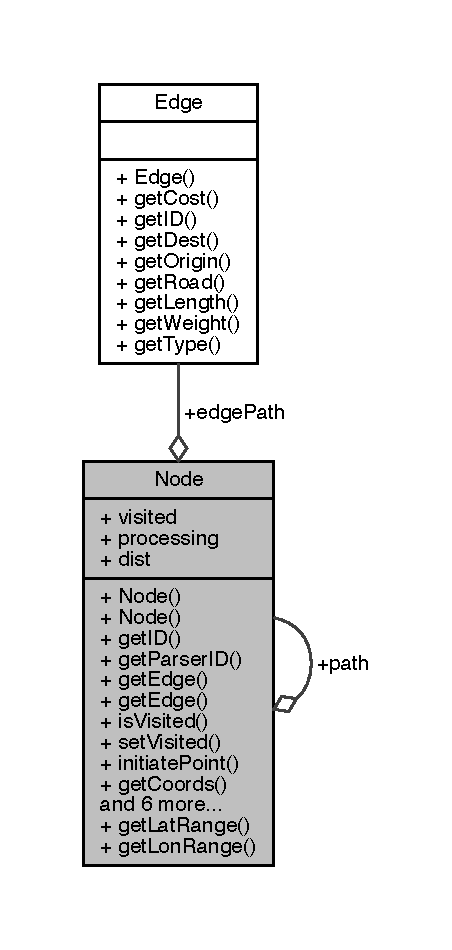
\includegraphics[width=217pt]{class_node__coll__graph}
\end{center}
\end{figure}
\subsection*{Public Member Functions}
\begin{DoxyCompactItemize}
\item 
\hyperlink{class_node_a3662f8e557681586b8a44df334dbdfaa}{Node} (istream \&input)
\item 
\hyperlink{class_node_aceb6d58ed1ee8fe95c532453a1f09ad2}{Node} (\hyperlink{_node_8hpp_a9d6265804805c2375068fd7484840dc6}{node\+\_\+id} id, \hyperlink{class_geographic_coords}{Geographic\+Coords} coords)
\item 
\hyperlink{_node_8hpp_a9d6265804805c2375068fd7484840dc6}{node\+\_\+id} \hyperlink{class_node_a5e319f5c050c46590bed81fc4dc54325}{get\+ID} () const
\item 
int \hyperlink{class_node_ab79cb8588caac0a2d0dd99d7e7dd2f28}{get\+Parser\+ID} () const
\item 
\hyperlink{class_edge}{Edge} $\ast$ \hyperlink{class_node_a108b79d820efdc2768a148e9308b3c31}{get\+Edge} () const
\item 
\hyperlink{class_edge}{Edge} $\ast$ \hyperlink{class_node_aaf31a7f0f8e4dea82e48b1b09b89c217}{get\+Edge} (\hyperlink{class_transport_a1879cecfed0d4238e5a7af6d085db317}{Transport\+::\+Type} type) const
\item 
bool \hyperlink{class_node_a97dd8f95e09a0516f8939627f94bd58e}{is\+Visited} () const
\item 
void \hyperlink{class_node_a9d8e32dbc9c7a9e488b08f4fd1ce178f}{set\+Visited} (bool state=true)
\item 
void \hyperlink{class_node_a599f948564fa9f0cb358fe030161eb1e}{initiate\+Point} (pair$<$ float, float $>$ lat\+Range, pair$<$ float, float $>$ lon\+Range)
\item 
\hyperlink{class_geographic_coords}{Geographic\+Coords} \hyperlink{class_node_a77aeb1b8ddb7776e097f5ad8a56bd0d0}{get\+Coords} () const
\item 
\hyperlink{class_point}{Point} \hyperlink{class_node_a73562032360227efd9fe93d07ab2475f}{get\+Point} () const
\item 
void \hyperlink{class_node_a9c981148bc1602d4388c6ea6428450c4}{add\+Edge} (\hyperlink{class_edge}{Edge} $\ast$ptr)
\item 
bool \hyperlink{class_node_a4c78d9813537ccfc829401f979176428}{remove\+Edge} (\hyperlink{class_edge}{Edge} $\ast$ptr)
\item 
void \hyperlink{class_node_a70d6617e33b3fc219f9d3c1bd48d7cca}{remove\+Edges\+To} (\hyperlink{_node_8hpp_a9d6265804805c2375068fd7484840dc6}{node\+\_\+id} id)
\item 
size\+\_\+t \hyperlink{class_node_abc4a69053f8f664c9b6a6a6bbe5d8c68}{get\+Num\+Edges} () const
\item 
const vector$<$ \hyperlink{class_edge}{Edge} $\ast$ $>$ \& \hyperlink{class_node_a10a4e5c428f496080172680cb20ea9e0}{get\+Edges} () const
\end{DoxyCompactItemize}
\subsection*{Static Public Member Functions}
\begin{DoxyCompactItemize}
\item 
static pair$<$ float, float $>$ \hyperlink{class_node_a258af43995af26e3ce9401bdd4948b30}{get\+Lat\+Range} ()
\item 
static pair$<$ float, float $>$ \hyperlink{class_node_a8533c4ac90cb7bc99895546b161e7d5a}{get\+Lon\+Range} ()
\end{DoxyCompactItemize}
\subsection*{Public Attributes}
\begin{DoxyCompactItemize}
\item 
bool \hyperlink{class_node_aa1bdec4e775fc578632e6a2dced9e251}{visited} = false
\item 
bool \hyperlink{class_node_ac54c0bde41664161566c30ccf4f8a53e}{processing} = false
\item 
float \hyperlink{class_node_ae7efda4ec8512d44445f058a479589d3}{dist} = numeric\+\_\+limits$<$float$>$\+::infinity()
\item 
\hyperlink{class_node}{Node} $\ast$ \hyperlink{class_node_a569c555f532e04a5ef976a54cd3c82a0}{path} = nullptr
\item 
\hyperlink{class_edge}{Edge} $\ast$ \hyperlink{class_node_a547c4e0904d03f97ca32a66408b11584}{edge\+Path} = nullptr
\end{DoxyCompactItemize}


\subsection{Detailed Description}
A class used to represent a \hyperlink{class_node}{Node} in a \hyperlink{class_graph}{Graph}. Every \hyperlink{class_node}{Node} has a unique ID, used to represent itself. Every \hyperlink{class_edge}{Edge} is also associated to a \hyperlink{class_road}{Road}, that contains more information about it. 

\subsection{Constructor \& Destructor Documentation}
\hypertarget{class_node_a3662f8e557681586b8a44df334dbdfaa}{}\label{class_node_a3662f8e557681586b8a44df334dbdfaa} 
\index{Node@{Node}!Node@{Node}}
\index{Node@{Node}!Node@{Node}}
\subsubsection{\texorpdfstring{Node()}{Node()}\hspace{0.1cm}{\footnotesize\ttfamily [1/2]}}
{\footnotesize\ttfamily Node\+::\+Node (\begin{DoxyParamCaption}\item[{istream \&}]{input }\end{DoxyParamCaption})}

\hyperlink{class_node}{Node}\textquotesingle{}s constructor from file. Creates a \hyperlink{class_node}{Node} with the data passed by the argument input stream.


\begin{DoxyParams}{Parameters}
{\em input} & The input stream to read from in order to build a \hyperlink{class_node}{Node} object. \\
\hline
\end{DoxyParams}
\hypertarget{class_node_aceb6d58ed1ee8fe95c532453a1f09ad2}{}\label{class_node_aceb6d58ed1ee8fe95c532453a1f09ad2} 
\index{Node@{Node}!Node@{Node}}
\index{Node@{Node}!Node@{Node}}
\subsubsection{\texorpdfstring{Node()}{Node()}\hspace{0.1cm}{\footnotesize\ttfamily [2/2]}}
{\footnotesize\ttfamily Node\+::\+Node (\begin{DoxyParamCaption}\item[{\hyperlink{_node_8hpp_a9d6265804805c2375068fd7484840dc6}{node\+\_\+id}}]{id,  }\item[{\hyperlink{class_geographic_coords}{Geographic\+Coords}}]{coords }\end{DoxyParamCaption})}

Incomplete constructor for \hyperlink{class_node}{Node}. Used only for \hyperlink{class_graph}{Graph}\textquotesingle{}s copy constructor, as all other attributes aren\textquotesingle{}t needed 

\subsection{Member Function Documentation}
\hypertarget{class_node_a9c981148bc1602d4388c6ea6428450c4}{}\label{class_node_a9c981148bc1602d4388c6ea6428450c4} 
\index{Node@{Node}!add\+Edge@{add\+Edge}}
\index{add\+Edge@{add\+Edge}!Node@{Node}}
\subsubsection{\texorpdfstring{add\+Edge()}{addEdge()}}
{\footnotesize\ttfamily void Node\+::add\+Edge (\begin{DoxyParamCaption}\item[{\hyperlink{class_edge}{Edge} $\ast$}]{ptr }\end{DoxyParamCaption})}

Function that associates the given \hyperlink{class_edge}{Edge} to the \hyperlink{class_node}{Node}.


\begin{DoxyParams}{Parameters}
{\em ptr} & \hyperlink{class_edge}{Edge} to be associated. \\
\hline
\end{DoxyParams}
\hypertarget{class_node_a77aeb1b8ddb7776e097f5ad8a56bd0d0}{}\label{class_node_a77aeb1b8ddb7776e097f5ad8a56bd0d0} 
\index{Node@{Node}!get\+Coords@{get\+Coords}}
\index{get\+Coords@{get\+Coords}!Node@{Node}}
\subsubsection{\texorpdfstring{get\+Coords()}{getCoords()}}
{\footnotesize\ttfamily \hyperlink{class_geographic_coords}{Geographic\+Coords} Node\+::get\+Coords (\begin{DoxyParamCaption}{ }\end{DoxyParamCaption}) const}

Getter for \hyperlink{class_node}{Node}\textquotesingle{}s Geographic Coordinates.

\begin{DoxyReturn}{Returns}
\hyperlink{class_node}{Node}\textquotesingle{}s Geographic Coordinates. 
\end{DoxyReturn}
\hypertarget{class_node_a108b79d820efdc2768a148e9308b3c31}{}\label{class_node_a108b79d820efdc2768a148e9308b3c31} 
\index{Node@{Node}!get\+Edge@{get\+Edge}}
\index{get\+Edge@{get\+Edge}!Node@{Node}}
\subsubsection{\texorpdfstring{get\+Edge()}{getEdge()}\hspace{0.1cm}{\footnotesize\ttfamily [1/2]}}
{\footnotesize\ttfamily \hyperlink{class_edge}{Edge} $\ast$ Node\+::get\+Edge (\begin{DoxyParamCaption}{ }\end{DoxyParamCaption}) const}

Getter for the \hyperlink{class_edge}{Edge} with the smallest weight, out of all the Edges associated to the \hyperlink{class_node}{Node}.

\begin{DoxyReturn}{Returns}
\hyperlink{class_edge}{Edge} associated to the \hyperlink{class_node}{Node}, with the smallest weight. 
\end{DoxyReturn}
\hypertarget{class_node_aaf31a7f0f8e4dea82e48b1b09b89c217}{}\label{class_node_aaf31a7f0f8e4dea82e48b1b09b89c217} 
\index{Node@{Node}!get\+Edge@{get\+Edge}}
\index{get\+Edge@{get\+Edge}!Node@{Node}}
\subsubsection{\texorpdfstring{get\+Edge()}{getEdge()}\hspace{0.1cm}{\footnotesize\ttfamily [2/2]}}
{\footnotesize\ttfamily \hyperlink{class_edge}{Edge} $\ast$ Node\+::get\+Edge (\begin{DoxyParamCaption}\item[{\hyperlink{class_transport_a1879cecfed0d4238e5a7af6d085db317}{Transport\+::\+Type}}]{type }\end{DoxyParamCaption}) const}

Getter for the \hyperlink{class_edge}{Edge} with the mean of \hyperlink{class_transport}{Transport} given, out of all the Edges associated to the \hyperlink{class_node}{Node}.

\begin{DoxyReturn}{Returns}
\hyperlink{class_edge}{Edge} associated to the \hyperlink{class_node}{Node}, whose mean of \hyperlink{class_transport}{Transport} is equal to the one given. 
\end{DoxyReturn}
\hypertarget{class_node_a10a4e5c428f496080172680cb20ea9e0}{}\label{class_node_a10a4e5c428f496080172680cb20ea9e0} 
\index{Node@{Node}!get\+Edges@{get\+Edges}}
\index{get\+Edges@{get\+Edges}!Node@{Node}}
\subsubsection{\texorpdfstring{get\+Edges()}{getEdges()}}
{\footnotesize\ttfamily const vector$<$ \hyperlink{class_edge}{Edge} $\ast$ $>$ \& Node\+::get\+Edges (\begin{DoxyParamCaption}{ }\end{DoxyParamCaption}) const}

Getter for all the Edges associated to the \hyperlink{class_node}{Node}.

\begin{DoxyReturn}{Returns}
vector of all the Edges associated to the \hyperlink{class_node}{Node}. 
\end{DoxyReturn}
\hypertarget{class_node_a5e319f5c050c46590bed81fc4dc54325}{}\label{class_node_a5e319f5c050c46590bed81fc4dc54325} 
\index{Node@{Node}!get\+ID@{get\+ID}}
\index{get\+ID@{get\+ID}!Node@{Node}}
\subsubsection{\texorpdfstring{get\+I\+D()}{getID()}}
{\footnotesize\ttfamily \hyperlink{_node_8hpp_a9d6265804805c2375068fd7484840dc6}{node\+\_\+id} Node\+::get\+ID (\begin{DoxyParamCaption}{ }\end{DoxyParamCaption}) const}

Getter for \hyperlink{class_node}{Node}\textquotesingle{}s ID. The ID is used to represent a \hyperlink{class_node}{Node}, since there are no two Nodes with the same ID.

\begin{DoxyReturn}{Returns}
\hyperlink{class_node}{Node}\textquotesingle{}s ID. 
\end{DoxyReturn}
\hypertarget{class_node_a258af43995af26e3ce9401bdd4948b30}{}\label{class_node_a258af43995af26e3ce9401bdd4948b30} 
\index{Node@{Node}!get\+Lat\+Range@{get\+Lat\+Range}}
\index{get\+Lat\+Range@{get\+Lat\+Range}!Node@{Node}}
\subsubsection{\texorpdfstring{get\+Lat\+Range()}{getLatRange()}}
{\footnotesize\ttfamily pair$<$ float, float $>$ Node\+::get\+Lat\+Range (\begin{DoxyParamCaption}{ }\end{DoxyParamCaption})\hspace{0.3cm}{\ttfamily [static]}}

Function the returns the Latitude Range.

\begin{DoxyReturn}{Returns}
Latitude range, where the first element is the minimum and the second the maximum. 
\end{DoxyReturn}
\hypertarget{class_node_a8533c4ac90cb7bc99895546b161e7d5a}{}\label{class_node_a8533c4ac90cb7bc99895546b161e7d5a} 
\index{Node@{Node}!get\+Lon\+Range@{get\+Lon\+Range}}
\index{get\+Lon\+Range@{get\+Lon\+Range}!Node@{Node}}
\subsubsection{\texorpdfstring{get\+Lon\+Range()}{getLonRange()}}
{\footnotesize\ttfamily pair$<$ float, float $>$ Node\+::get\+Lon\+Range (\begin{DoxyParamCaption}{ }\end{DoxyParamCaption})\hspace{0.3cm}{\ttfamily [static]}}

Function the returns the Longitude Range.

\begin{DoxyReturn}{Returns}
Longitude range, where the first element is the minimum and the second the maximum. 
\end{DoxyReturn}
\hypertarget{class_node_abc4a69053f8f664c9b6a6a6bbe5d8c68}{}\label{class_node_abc4a69053f8f664c9b6a6a6bbe5d8c68} 
\index{Node@{Node}!get\+Num\+Edges@{get\+Num\+Edges}}
\index{get\+Num\+Edges@{get\+Num\+Edges}!Node@{Node}}
\subsubsection{\texorpdfstring{get\+Num\+Edges()}{getNumEdges()}}
{\footnotesize\ttfamily size\+\_\+t Node\+::get\+Num\+Edges (\begin{DoxyParamCaption}{ }\end{DoxyParamCaption}) const}

Getter for the number of Edges associated to the \hyperlink{class_node}{Node}.

\begin{DoxyReturn}{Returns}
Number of Edges associated to the \hyperlink{class_node}{Node}. 
\end{DoxyReturn}
\hypertarget{class_node_ab79cb8588caac0a2d0dd99d7e7dd2f28}{}\label{class_node_ab79cb8588caac0a2d0dd99d7e7dd2f28} 
\index{Node@{Node}!get\+Parser\+ID@{get\+Parser\+ID}}
\index{get\+Parser\+ID@{get\+Parser\+ID}!Node@{Node}}
\subsubsection{\texorpdfstring{get\+Parser\+I\+D()}{getParserID()}}
{\footnotesize\ttfamily int Node\+::get\+Parser\+ID (\begin{DoxyParamCaption}{ }\end{DoxyParamCaption}) const}

Getter for \hyperlink{class_node}{Node}\textquotesingle{}s Parser ID. The parser ID is also used to represent a \hyperlink{class_node}{Node}, since there are no two Nodes with the same parser ID. This ID is sequential.

\begin{DoxyReturn}{Returns}
\hyperlink{class_node}{Node}\textquotesingle{}s parser ID. 
\end{DoxyReturn}
\hypertarget{class_node_a73562032360227efd9fe93d07ab2475f}{}\label{class_node_a73562032360227efd9fe93d07ab2475f} 
\index{Node@{Node}!get\+Point@{get\+Point}}
\index{get\+Point@{get\+Point}!Node@{Node}}
\subsubsection{\texorpdfstring{get\+Point()}{getPoint()}}
{\footnotesize\ttfamily \hyperlink{class_point}{Point} Node\+::get\+Point (\begin{DoxyParamCaption}{ }\end{DoxyParamCaption}) const}

Getter for \hyperlink{class_node}{Node}\textquotesingle{}s correspondent \hyperlink{class_point}{Point} in a 2D Plane.

\begin{DoxyReturn}{Returns}
\hyperlink{class_node}{Node}\textquotesingle{}s correspondent \hyperlink{class_point}{Point}. 
\end{DoxyReturn}
\hypertarget{class_node_a599f948564fa9f0cb358fe030161eb1e}{}\label{class_node_a599f948564fa9f0cb358fe030161eb1e} 
\index{Node@{Node}!initiate\+Point@{initiate\+Point}}
\index{initiate\+Point@{initiate\+Point}!Node@{Node}}
\subsubsection{\texorpdfstring{initiate\+Point()}{initiatePoint()}}
{\footnotesize\ttfamily void Node\+::initiate\+Point (\begin{DoxyParamCaption}\item[{pair$<$ float, float $>$}]{lat\+Range,  }\item[{pair$<$ float, float $>$}]{lon\+Range }\end{DoxyParamCaption})}

Builds the \hyperlink{class_node}{Node}\textquotesingle{}s correspondent \hyperlink{class_point}{Point} in a 2D Plane.


\begin{DoxyParams}{Parameters}
{\em lat\+Range} & Latitude range, where the first element is the minimum and the second the maximum. \\
\hline
{\em lon\+Range} & Longitude range, where the first element is the minimum and the second the maximum. \\
\hline
\end{DoxyParams}
\hypertarget{class_node_a97dd8f95e09a0516f8939627f94bd58e}{}\label{class_node_a97dd8f95e09a0516f8939627f94bd58e} 
\index{Node@{Node}!is\+Visited@{is\+Visited}}
\index{is\+Visited@{is\+Visited}!Node@{Node}}
\subsubsection{\texorpdfstring{is\+Visited()}{isVisited()}}
{\footnotesize\ttfamily bool Node\+::is\+Visited (\begin{DoxyParamCaption}{ }\end{DoxyParamCaption}) const}

Getter for flag that if set \hyperlink{class_node}{Node}\textquotesingle{}s has already been visited in path, otherwise has not.

\begin{DoxyReturn}{Returns}
Value of the Flag. 
\end{DoxyReturn}
\hypertarget{class_node_a4c78d9813537ccfc829401f979176428}{}\label{class_node_a4c78d9813537ccfc829401f979176428} 
\index{Node@{Node}!remove\+Edge@{remove\+Edge}}
\index{remove\+Edge@{remove\+Edge}!Node@{Node}}
\subsubsection{\texorpdfstring{remove\+Edge()}{removeEdge()}}
{\footnotesize\ttfamily bool Node\+::remove\+Edge (\begin{DoxyParamCaption}\item[{\hyperlink{class_edge}{Edge} $\ast$}]{ptr }\end{DoxyParamCaption})}

Function that removes the \hyperlink{class_edge}{Edge} given from the \hyperlink{class_node}{Node}\textquotesingle{}s associated Edges.


\begin{DoxyParams}{Parameters}
{\em ptr} & \hyperlink{class_edge}{Edge} to be removed.\\
\hline
\end{DoxyParams}
\begin{DoxyReturn}{Returns}
True if the \hyperlink{class_edge}{Edge} was removed, false otherwise. 
\end{DoxyReturn}
\hypertarget{class_node_a70d6617e33b3fc219f9d3c1bd48d7cca}{}\label{class_node_a70d6617e33b3fc219f9d3c1bd48d7cca} 
\index{Node@{Node}!remove\+Edges\+To@{remove\+Edges\+To}}
\index{remove\+Edges\+To@{remove\+Edges\+To}!Node@{Node}}
\subsubsection{\texorpdfstring{remove\+Edges\+To()}{removeEdgesTo()}}
{\footnotesize\ttfamily void Node\+::remove\+Edges\+To (\begin{DoxyParamCaption}\item[{\hyperlink{_node_8hpp_a9d6265804805c2375068fd7484840dc6}{node\+\_\+id}}]{id }\end{DoxyParamCaption})}

Function that removes the Edges whose destiny \hyperlink{class_node}{Node} is the given \hyperlink{class_node}{Node}.


\begin{DoxyParams}{Parameters}
{\em id} & ID of the \hyperlink{class_node}{Node} used to updated the Edges. \\
\hline
\end{DoxyParams}
\hypertarget{class_node_a9d8e32dbc9c7a9e488b08f4fd1ce178f}{}\label{class_node_a9d8e32dbc9c7a9e488b08f4fd1ce178f} 
\index{Node@{Node}!set\+Visited@{set\+Visited}}
\index{set\+Visited@{set\+Visited}!Node@{Node}}
\subsubsection{\texorpdfstring{set\+Visited()}{setVisited()}}
{\footnotesize\ttfamily void Node\+::set\+Visited (\begin{DoxyParamCaption}\item[{bool}]{state = {\ttfamily true} }\end{DoxyParamCaption})}

Function changes the correspondent flag value. If set \hyperlink{class_node}{Node}\textquotesingle{}s has already been visited in path, otherwise has not. If no value is given, it defaults to true.


\begin{DoxyParams}{Parameters}
{\em state} & State to change the flag to. \\
\hline
\end{DoxyParams}


\subsection{Member Data Documentation}
\hypertarget{class_node_ae7efda4ec8512d44445f058a479589d3}{}\label{class_node_ae7efda4ec8512d44445f058a479589d3} 
\index{Node@{Node}!dist@{dist}}
\index{dist@{dist}!Node@{Node}}
\subsubsection{\texorpdfstring{dist}{dist}}
{\footnotesize\ttfamily float Node\+::dist = numeric\+\_\+limits$<$float$>$\+::infinity()}

float dist. Distance used for calculus in the Dijkstra algorithm. Represents the minimum distance from the \hyperlink{class_node}{Node} to the origin \hyperlink{class_node}{Node}. \hypertarget{class_node_a547c4e0904d03f97ca32a66408b11584}{}\label{class_node_a547c4e0904d03f97ca32a66408b11584} 
\index{Node@{Node}!edge\+Path@{edge\+Path}}
\index{edge\+Path@{edge\+Path}!Node@{Node}}
\subsubsection{\texorpdfstring{edge\+Path}{edgePath}}
{\footnotesize\ttfamily \hyperlink{class_edge}{Edge}$\ast$ Node\+::edge\+Path = nullptr}

Edge$\ast$ path. Pointer to the \hyperlink{class_edge}{Edge}, linking the \hyperlink{class_node}{Node} to the previous one in the path. \hypertarget{class_node_a569c555f532e04a5ef976a54cd3c82a0}{}\label{class_node_a569c555f532e04a5ef976a54cd3c82a0} 
\index{Node@{Node}!path@{path}}
\index{path@{path}!Node@{Node}}
\subsubsection{\texorpdfstring{path}{path}}
{\footnotesize\ttfamily \hyperlink{class_node}{Node}$\ast$ Node\+::path = nullptr}

Node$\ast$ path. Pointer to the previous \hyperlink{class_node}{Node} in the path. \hypertarget{class_node_ac54c0bde41664161566c30ccf4f8a53e}{}\label{class_node_ac54c0bde41664161566c30ccf4f8a53e} 
\index{Node@{Node}!processing@{processing}}
\index{processing@{processing}!Node@{Node}}
\subsubsection{\texorpdfstring{processing}{processing}}
{\footnotesize\ttfamily bool Node\+::processing = false}

bool processing. Flag\+: If true, \hyperlink{class_node}{Node} is being processed in the Dijkstra algorithm, otherwise is not. \hypertarget{class_node_aa1bdec4e775fc578632e6a2dced9e251}{}\label{class_node_aa1bdec4e775fc578632e6a2dced9e251} 
\index{Node@{Node}!visited@{visited}}
\index{visited@{visited}!Node@{Node}}
\subsubsection{\texorpdfstring{visited}{visited}}
{\footnotesize\ttfamily bool Node\+::visited = false}

bool visited. Flag\+: If true, \hyperlink{class_node}{Node} was already visited in the path, otherwise was not. 

The documentation for this class was generated from the following files\+:\begin{DoxyCompactItemize}
\item 
\hyperlink{_node_8hpp}{Node.\+hpp}\item 
\hyperlink{_node_8cpp}{Node.\+cpp}\end{DoxyCompactItemize}

\hypertarget{structnode__greater__than}{}\section{node\+\_\+greater\+\_\+than Struct Reference}
\label{structnode__greater__than}\index{node\+\_\+greater\+\_\+than@{node\+\_\+greater\+\_\+than}}


Collaboration diagram for node\+\_\+greater\+\_\+than\+:\nopagebreak
\begin{figure}[H]
\begin{center}
\leavevmode
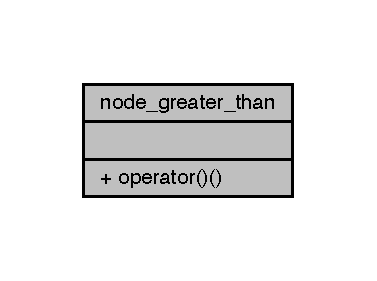
\includegraphics[width=181pt]{structnode__greater__than__coll__graph}
\end{center}
\end{figure}
\subsection*{Public Member Functions}
\begin{DoxyCompactItemize}
\item 
bool \hyperlink{structnode__greater__than_ac91d8c047b4c548f2c1ddf95af5a8f6d}{operator()} (\hyperlink{class_node}{Node} $\ast$a, \hyperlink{class_node}{Node} $\ast$b) const
\end{DoxyCompactItemize}


\subsection{Member Function Documentation}
\hypertarget{structnode__greater__than_ac91d8c047b4c548f2c1ddf95af5a8f6d}{}\label{structnode__greater__than_ac91d8c047b4c548f2c1ddf95af5a8f6d} 
\index{node\+\_\+greater\+\_\+than@{node\+\_\+greater\+\_\+than}!operator()@{operator()}}
\index{operator()@{operator()}!node\+\_\+greater\+\_\+than@{node\+\_\+greater\+\_\+than}}
\subsubsection{\texorpdfstring{operator()()}{operator()()}}
{\footnotesize\ttfamily bool node\+\_\+greater\+\_\+than\+::operator() (\begin{DoxyParamCaption}\item[{\hyperlink{class_node}{Node} $\ast$}]{a,  }\item[{\hyperlink{class_node}{Node} $\ast$}]{b }\end{DoxyParamCaption}) const\hspace{0.3cm}{\ttfamily [inline]}}



The documentation for this struct was generated from the following file\+:\begin{DoxyCompactItemize}
\item 
\hyperlink{_graph_8cpp}{Graph.\+cpp}\end{DoxyCompactItemize}

\hypertarget{structnode__pair__greater__than}{}\section{node\+\_\+pair\+\_\+greater\+\_\+than Struct Reference}
\label{structnode__pair__greater__than}\index{node\+\_\+pair\+\_\+greater\+\_\+than@{node\+\_\+pair\+\_\+greater\+\_\+than}}


Collaboration diagram for node\+\_\+pair\+\_\+greater\+\_\+than\+:\nopagebreak
\begin{figure}[H]
\begin{center}
\leavevmode
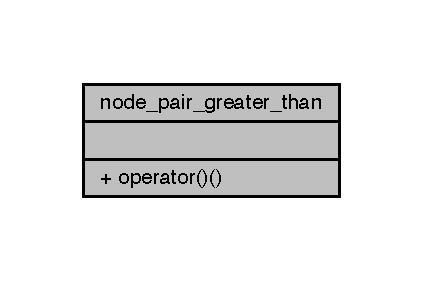
\includegraphics[width=203pt]{structnode__pair__greater__than__coll__graph}
\end{center}
\end{figure}
\subsection*{Public Member Functions}
\begin{DoxyCompactItemize}
\item 
bool \hyperlink{structnode__pair__greater__than_aefc537db2afdf9b3b89469adaaeea00b}{operator()} (const pair$<$ \hyperlink{class_node}{Node} $\ast$, unsigned $>$ \&p1, const pair$<$ \hyperlink{class_node}{Node} $\ast$, unsigned $>$ \&p2)
\end{DoxyCompactItemize}


\subsection{Member Function Documentation}
\hypertarget{structnode__pair__greater__than_aefc537db2afdf9b3b89469adaaeea00b}{}\label{structnode__pair__greater__than_aefc537db2afdf9b3b89469adaaeea00b} 
\index{node\+\_\+pair\+\_\+greater\+\_\+than@{node\+\_\+pair\+\_\+greater\+\_\+than}!operator()@{operator()}}
\index{operator()@{operator()}!node\+\_\+pair\+\_\+greater\+\_\+than@{node\+\_\+pair\+\_\+greater\+\_\+than}}
\subsubsection{\texorpdfstring{operator()()}{operator()()}}
{\footnotesize\ttfamily bool node\+\_\+pair\+\_\+greater\+\_\+than\+::operator() (\begin{DoxyParamCaption}\item[{const pair$<$ \hyperlink{class_node}{Node} $\ast$, unsigned $>$ \&}]{p1,  }\item[{const pair$<$ \hyperlink{class_node}{Node} $\ast$, unsigned $>$ \&}]{p2 }\end{DoxyParamCaption})\hspace{0.3cm}{\ttfamily [inline]}}



The documentation for this struct was generated from the following file\+:\begin{DoxyCompactItemize}
\item 
\hyperlink{_graph_8cpp}{Graph.\+cpp}\end{DoxyCompactItemize}

\hypertarget{class_point}{}\section{Point Class Reference}
\label{class_point}\index{Point@{Point}}


{\ttfamily \#include $<$Coordinates.\+hpp$>$}

\subsection*{Public Member Functions}
\begin{DoxyCompactItemize}
\item 
\hyperlink{class_point_a257415ad611a16bb73628efcdb87d0fd}{Point} ()=default
\item 
\hyperlink{class_point_a30bc8409287de4f43e160664be834636}{Point} (float x, float y)
\item 
float \hyperlink{class_point_a29c44ec7c7279e02629645a06cdaf7d5}{getX} () const
\item 
float \hyperlink{class_point_a2371ffadbe245d12a8f556d0a976521b}{getY} () const
\end{DoxyCompactItemize}
\subsection*{Static Public Member Functions}
\begin{DoxyCompactItemize}
\item 
static float \hyperlink{class_point_a1dbe2026f242cd96843ea14a67e8a2c3}{get\+Distance} (const \hyperlink{class_point}{Point} \&p1, const \hyperlink{class_point}{Point} \&p2)
\end{DoxyCompactItemize}


\subsection{Detailed Description}
A class used to represent a \hyperlink{class_point}{Point} in a 2D Plane. Every \hyperlink{class_point}{Point} is represented as (x, y) in cartesian coordinates. 

\subsection{Constructor \& Destructor Documentation}
\hypertarget{class_point_a257415ad611a16bb73628efcdb87d0fd}{}\label{class_point_a257415ad611a16bb73628efcdb87d0fd} 
\index{Point@{Point}!Point@{Point}}
\index{Point@{Point}!Point@{Point}}
\subsubsection{\texorpdfstring{Point()}{Point()}\hspace{0.1cm}{\footnotesize\ttfamily [1/2]}}
{\footnotesize\ttfamily Point\+::\+Point (\begin{DoxyParamCaption}{ }\end{DoxyParamCaption})\hspace{0.3cm}{\ttfamily [default]}}

Explicit Default constructor. \hypertarget{class_point_a30bc8409287de4f43e160664be834636}{}\label{class_point_a30bc8409287de4f43e160664be834636} 
\index{Point@{Point}!Point@{Point}}
\index{Point@{Point}!Point@{Point}}
\subsubsection{\texorpdfstring{Point()}{Point()}\hspace{0.1cm}{\footnotesize\ttfamily [2/2]}}
{\footnotesize\ttfamily Point\+::\+Point (\begin{DoxyParamCaption}\item[{float}]{x,  }\item[{float}]{y }\end{DoxyParamCaption})}

\hyperlink{class_point}{Point}\textquotesingle{}s constructor. Creates a \hyperlink{class_point}{Point} with the given coordinates.


\begin{DoxyParams}{Parameters}
{\em x} & \hyperlink{class_point}{Point}\textquotesingle{}s coordinate value on the horizontal axis. \\
\hline
{\em y} & \hyperlink{class_point}{Point}\textquotesingle{}s coordinate value on the vertical axis. \\
\hline
\end{DoxyParams}


\subsection{Member Function Documentation}
\hypertarget{class_point_a1dbe2026f242cd96843ea14a67e8a2c3}{}\label{class_point_a1dbe2026f242cd96843ea14a67e8a2c3} 
\index{Point@{Point}!get\+Distance@{get\+Distance}}
\index{get\+Distance@{get\+Distance}!Point@{Point}}
\subsubsection{\texorpdfstring{get\+Distance()}{getDistance()}}
{\footnotesize\ttfamily float Point\+::get\+Distance (\begin{DoxyParamCaption}\item[{const \hyperlink{class_point}{Point} \&}]{p1,  }\item[{const \hyperlink{class_point}{Point} \&}]{p2 }\end{DoxyParamCaption})\hspace{0.3cm}{\ttfamily [static]}}

Function used to calculate the distance between two given Points. Makes use of the Pythagorean Theorem Formula


\begin{DoxyParams}{Parameters}
{\em p1} & \hyperlink{class_point}{Point} to be used in the calculus. \\
\hline
{\em p2} & \hyperlink{class_point}{Point} to be used in the calculus.\\
\hline
\end{DoxyParams}
\begin{DoxyReturn}{Returns}
the distance between the two Points. 
\end{DoxyReturn}
\hypertarget{class_point_a29c44ec7c7279e02629645a06cdaf7d5}{}\label{class_point_a29c44ec7c7279e02629645a06cdaf7d5} 
\index{Point@{Point}!getX@{getX}}
\index{getX@{getX}!Point@{Point}}
\subsubsection{\texorpdfstring{get\+X()}{getX()}}
{\footnotesize\ttfamily float Point\+::getX (\begin{DoxyParamCaption}{ }\end{DoxyParamCaption}) const}

Getter for coordinate value on the horizontal axis.

\begin{DoxyReturn}{Returns}
coordinate value on the horizontal axis. 
\end{DoxyReturn}
\hypertarget{class_point_a2371ffadbe245d12a8f556d0a976521b}{}\label{class_point_a2371ffadbe245d12a8f556d0a976521b} 
\index{Point@{Point}!getY@{getY}}
\index{getY@{getY}!Point@{Point}}
\subsubsection{\texorpdfstring{get\+Y()}{getY()}}
{\footnotesize\ttfamily float Point\+::getY (\begin{DoxyParamCaption}{ }\end{DoxyParamCaption}) const}

Getter for coordinate value on the vertical axis.

\begin{DoxyReturn}{Returns}
coordinate value on the vertical axis. 
\end{DoxyReturn}


The documentation for this class was generated from the following files\+:\begin{DoxyCompactItemize}
\item 
Coordinates.\+hpp\item 
Coordinates.\+cpp\end{DoxyCompactItemize}

\hypertarget{class_road}{}\section{Road Class Reference}
\label{class_road}\index{Road@{Road}}


{\ttfamily \#include $<$Road.\+hpp$>$}

\subsection*{Public Member Functions}
\begin{DoxyCompactItemize}
\item 
\hyperlink{class_road_a4bd6abfd59885bb839dff8642b32db92}{Road} (road\+\_\+id id, string name, bool two\+Way)
\item 
\hyperlink{class_road_a96d7a3bee9ce4ea3ed6ed8eb24298085}{Road} (istream \&input)
\item 
road\+\_\+id \hyperlink{class_road_a4e0440c1d5bf11800f0df3c50dcb4b92}{get\+ID} () const
\item 
string \hyperlink{class_road_ae7c959eda8a11bc859ab5de5e278b735}{get\+Name} () const
\item 
bool \hyperlink{class_road_a9c412810b3a630a759f199c60f7f1cc6}{is\+Two\+Way} () const
\item 
bool \hyperlink{class_road_a7a691f98e8bd53299ed2539de1e4d13c}{add\+Edge} (\hyperlink{class_edge}{Edge} $\ast$ptr)
\item 
const set$<$ \hyperlink{class_edge}{Edge} $\ast$ $>$ \hyperlink{class_road_a03fb1c0a74b860e4be6c951154add098}{get\+Edges} ()
\end{DoxyCompactItemize}


\subsection{Detailed Description}
Class used to represent a \hyperlink{class_road}{Road}. Every \hyperlink{class_road}{Road} has a unique ID, a name, and a flag regarding the direction of the \hyperlink{class_road}{Road}. Roads can also be associated to different Edges. 

\subsection{Constructor \& Destructor Documentation}
\hypertarget{class_road_a4bd6abfd59885bb839dff8642b32db92}{}\label{class_road_a4bd6abfd59885bb839dff8642b32db92} 
\index{Road@{Road}!Road@{Road}}
\index{Road@{Road}!Road@{Road}}
\subsubsection{\texorpdfstring{Road()}{Road()}\hspace{0.1cm}{\footnotesize\ttfamily [1/2]}}
{\footnotesize\ttfamily Road\+::\+Road (\begin{DoxyParamCaption}\item[{road\+\_\+id}]{id,  }\item[{string}]{name,  }\item[{bool}]{two\+Way }\end{DoxyParamCaption})}

\hyperlink{class_road}{Road}\textquotesingle{}s constructor. Creates a \hyperlink{class_road}{Road} with the given ID, name and flag If the flag is set traffic goes both ways, otherwise traffic only goes one way.


\begin{DoxyParams}{Parameters}
{\em id} & \hyperlink{class_road}{Road}\textquotesingle{}s unique ID. \\
\hline
{\em name} & \hyperlink{class_road}{Road}\textquotesingle{}s Name. \\
\hline
{\em two\+Way} & Flag regarding \hyperlink{class_road}{Road}\textquotesingle{}s traffic direction. \\
\hline
\end{DoxyParams}
\hypertarget{class_road_a96d7a3bee9ce4ea3ed6ed8eb24298085}{}\label{class_road_a96d7a3bee9ce4ea3ed6ed8eb24298085} 
\index{Road@{Road}!Road@{Road}}
\index{Road@{Road}!Road@{Road}}
\subsubsection{\texorpdfstring{Road()}{Road()}\hspace{0.1cm}{\footnotesize\ttfamily [2/2]}}
{\footnotesize\ttfamily Road\+::\+Road (\begin{DoxyParamCaption}\item[{istream \&}]{input }\end{DoxyParamCaption})}

\hyperlink{class_road}{Road}\textquotesingle{}s constructor from file. Creates a \hyperlink{class_road}{Road} with the data passed by the argument input stream.


\begin{DoxyParams}{Parameters}
{\em input} & The input stream to read from in order to build a \hyperlink{class_road}{Road} object. \\
\hline
\end{DoxyParams}


\subsection{Member Function Documentation}
\hypertarget{class_road_a7a691f98e8bd53299ed2539de1e4d13c}{}\label{class_road_a7a691f98e8bd53299ed2539de1e4d13c} 
\index{Road@{Road}!add\+Edge@{add\+Edge}}
\index{add\+Edge@{add\+Edge}!Road@{Road}}
\subsubsection{\texorpdfstring{add\+Edge()}{addEdge()}}
{\footnotesize\ttfamily bool Road\+::add\+Edge (\begin{DoxyParamCaption}\item[{\hyperlink{class_edge}{Edge} $\ast$}]{ptr }\end{DoxyParamCaption})}

Function used to associate an \hyperlink{class_edge}{Edge} to the \hyperlink{class_road}{Road}.


\begin{DoxyParams}{Parameters}
{\em ptr} & to be associated\\
\hline
\end{DoxyParams}
\begin{DoxyReturn}{Returns}
true if the \hyperlink{class_edge}{Edge} was added to the container of all associated Edges, false otherwise. 
\end{DoxyReturn}
\hypertarget{class_road_a03fb1c0a74b860e4be6c951154add098}{}\label{class_road_a03fb1c0a74b860e4be6c951154add098} 
\index{Road@{Road}!get\+Edges@{get\+Edges}}
\index{get\+Edges@{get\+Edges}!Road@{Road}}
\subsubsection{\texorpdfstring{get\+Edges()}{getEdges()}}
{\footnotesize\ttfamily const set$<$ \hyperlink{class_edge}{Edge} $\ast$ $>$ Road\+::get\+Edges (\begin{DoxyParamCaption}{ }\end{DoxyParamCaption})}

Getter for all Edges associated to the \hyperlink{class_road}{Road}.

\begin{DoxyReturn}{Returns}
Set that contains all Edges associated to the \hyperlink{class_road}{Road}. 
\end{DoxyReturn}
\hypertarget{class_road_a4e0440c1d5bf11800f0df3c50dcb4b92}{}\label{class_road_a4e0440c1d5bf11800f0df3c50dcb4b92} 
\index{Road@{Road}!get\+ID@{get\+ID}}
\index{get\+ID@{get\+ID}!Road@{Road}}
\subsubsection{\texorpdfstring{get\+I\+D()}{getID()}}
{\footnotesize\ttfamily road\+\_\+id Road\+::get\+ID (\begin{DoxyParamCaption}{ }\end{DoxyParamCaption}) const}

Getter for \hyperlink{class_road}{Road}\textquotesingle{}s ID. The ID is used to represent a \hyperlink{class_road}{Road}, since there are no two Roads with the same ID.

\begin{DoxyReturn}{Returns}
The \hyperlink{class_road}{Road}\textquotesingle{}s ID. 
\end{DoxyReturn}
\hypertarget{class_road_ae7c959eda8a11bc859ab5de5e278b735}{}\label{class_road_ae7c959eda8a11bc859ab5de5e278b735} 
\index{Road@{Road}!get\+Name@{get\+Name}}
\index{get\+Name@{get\+Name}!Road@{Road}}
\subsubsection{\texorpdfstring{get\+Name()}{getName()}}
{\footnotesize\ttfamily string Road\+::get\+Name (\begin{DoxyParamCaption}{ }\end{DoxyParamCaption}) const}

Getter for \hyperlink{class_road}{Road}\textquotesingle{}s Name.

\begin{DoxyReturn}{Returns}
The \hyperlink{class_road}{Road}\textquotesingle{}s name. 
\end{DoxyReturn}
\hypertarget{class_road_a9c412810b3a630a759f199c60f7f1cc6}{}\label{class_road_a9c412810b3a630a759f199c60f7f1cc6} 
\index{Road@{Road}!is\+Two\+Way@{is\+Two\+Way}}
\index{is\+Two\+Way@{is\+Two\+Way}!Road@{Road}}
\subsubsection{\texorpdfstring{is\+Two\+Way()}{isTwoWay()}}
{\footnotesize\ttfamily bool Road\+::is\+Two\+Way (\begin{DoxyParamCaption}{ }\end{DoxyParamCaption}) const}

Getter for \hyperlink{class_road}{Road}\textquotesingle{}s flag regarding its direction. If the flag is set traffic goes both ways, otherwise traffic only goes one way.

\begin{DoxyReturn}{Returns}
flag regarding \hyperlink{class_road}{Road}\textquotesingle{}s direction. 
\end{DoxyReturn}


The documentation for this class was generated from the following files\+:\begin{DoxyCompactItemize}
\item 
Road.\+hpp\item 
Road.\+cpp\end{DoxyCompactItemize}

\hypertarget{class_transport}{}\section{Transport Class Reference}
\label{class_transport}\index{Transport@{Transport}}


{\ttfamily \#include $<$Transport.\+hpp$>$}

\subsection*{Public Types}
\begin{DoxyCompactItemize}
\item 
enum \hyperlink{class_transport_a1879cecfed0d4238e5a7af6d085db317}{Type} \{ {\bfseries F\+O\+OT}, 
{\bfseries B\+US}, 
{\bfseries S\+U\+B\+W\+AY}
 \}
\end{DoxyCompactItemize}
\subsection*{Public Member Functions}
\begin{DoxyCompactItemize}
\item 
unsigned int \hyperlink{class_transport_ae9b8f3d27331e429160827194e32bde1}{get\+Vel} (\hyperlink{class_transport_a1879cecfed0d4238e5a7af6d085db317}{Type} t) const
\item 
unsigned int \hyperlink{class_transport_a943eecabe9f2435fcbf2bd3a41a4ea3a}{get\+Cost} (\hyperlink{class_transport_a1879cecfed0d4238e5a7af6d085db317}{Type} t) const
\end{DoxyCompactItemize}
\subsection*{Static Public Member Functions}
\begin{DoxyCompactItemize}
\item 
static \hyperlink{class_transport}{Transport} $\ast$ \hyperlink{class_transport_a2265878b8225332acf586bece5f1b324}{get\+Instance} ()
\end{DoxyCompactItemize}


\subsection{Detailed Description}
Class used to represent means of \hyperlink{class_transport}{Transport}. The difference between means of \hyperlink{class_transport}{Transport} is the velocity with which they can traverse a certain route. 

\subsection{Member Enumeration Documentation}
\hypertarget{class_transport_a1879cecfed0d4238e5a7af6d085db317}{}\label{class_transport_a1879cecfed0d4238e5a7af6d085db317} 
\index{Transport@{Transport}!Type@{Type}}
\index{Type@{Type}!Transport@{Transport}}
\subsubsection{\texorpdfstring{Type}{Type}}
{\footnotesize\ttfamily enum \hyperlink{class_transport_a1879cecfed0d4238e5a7af6d085db317}{Transport\+::\+Type}}

Enumeration containing the different means of transport. 

\subsection{Member Function Documentation}
\hypertarget{class_transport_a943eecabe9f2435fcbf2bd3a41a4ea3a}{}\label{class_transport_a943eecabe9f2435fcbf2bd3a41a4ea3a} 
\index{Transport@{Transport}!get\+Cost@{get\+Cost}}
\index{get\+Cost@{get\+Cost}!Transport@{Transport}}
\subsubsection{\texorpdfstring{get\+Cost()}{getCost()}}
{\footnotesize\ttfamily unsigned int Transport\+::get\+Cost (\begin{DoxyParamCaption}\item[{\hyperlink{class_transport_a1879cecfed0d4238e5a7af6d085db317}{Type}}]{t }\end{DoxyParamCaption}) const}

Getter for the cost of the current mean of \hyperlink{class_transport}{Transport}, in cents per Kilometer.

\begin{DoxyReturn}{Returns}
Cost of the current mean of \hyperlink{class_transport}{Transport}. 
\end{DoxyReturn}
\hypertarget{class_transport_a2265878b8225332acf586bece5f1b324}{}\label{class_transport_a2265878b8225332acf586bece5f1b324} 
\index{Transport@{Transport}!get\+Instance@{get\+Instance}}
\index{get\+Instance@{get\+Instance}!Transport@{Transport}}
\subsubsection{\texorpdfstring{get\+Instance()}{getInstance()}}
{\footnotesize\ttfamily \hyperlink{class_transport}{Transport} $\ast$ Transport\+::get\+Instance (\begin{DoxyParamCaption}{ }\end{DoxyParamCaption})\hspace{0.3cm}{\ttfamily [static]}}

Getter for the current mean of \hyperlink{class_transport}{Transport}. If no mean of transport exists, a new one is created.

\begin{DoxyReturn}{Returns}
The current mean of \hyperlink{class_transport}{Transport}. 
\end{DoxyReturn}
\hypertarget{class_transport_ae9b8f3d27331e429160827194e32bde1}{}\label{class_transport_ae9b8f3d27331e429160827194e32bde1} 
\index{Transport@{Transport}!get\+Vel@{get\+Vel}}
\index{get\+Vel@{get\+Vel}!Transport@{Transport}}
\subsubsection{\texorpdfstring{get\+Vel()}{getVel()}}
{\footnotesize\ttfamily unsigned int Transport\+::get\+Vel (\begin{DoxyParamCaption}\item[{\hyperlink{class_transport_a1879cecfed0d4238e5a7af6d085db317}{Transport\+::\+Type}}]{t }\end{DoxyParamCaption}) const}

Getter for the velocity of the current mean of \hyperlink{class_transport}{Transport}.

\begin{DoxyReturn}{Returns}
Velocity of the current mean of \hyperlink{class_transport}{Transport}. 
\end{DoxyReturn}


The documentation for this class was generated from the following files\+:\begin{DoxyCompactItemize}
\item 
Transport.\+hpp\item 
Transport.\+cpp\end{DoxyCompactItemize}

%--- End generated contents ---

% Index
\backmatter
\newpage
\phantomsection
\clearemptydoublepage
\addcontentsline{toc}{chapter}{Index}
\printindex

\end{document}
